\myChapter{Contribution~: enrichissement g\'eospatial g\'en\'erique et pr\'ediction du risque PFAS}{Contribution~: enrichissement g\'eospatial g\'en\'erique et pr\'ediction du risque PFAS}
\label{chap:contribution}
\myMiniToc{section}{Sommaire}

% =========================================================
\mySection{Introduction}{}
\label{sec:contrib-intro}
% =========================================================

Le chapitre~\ref{chap:etat-art} a d\'egag\'e quatre lacunes structurelles dans la litt\'erature de pr\'ediction des PFAS par apprentissage automatique (section~\ref{sec:chap2-lacunes})~: la structure relationnelle entre forages voisins, panaches et sources communes reste sous-exploit\'ee (L1)~; un biais d'\'evaluation circulaire appara\^it lorsque des concentrations PFAS mesur\'ees se glissent dans les variables, sans s\'eparer clairement le mode pr\'edictif du mode confirmatoire (L2)~; la transf\'erabilit\'e g\'eographique est rarement valid\'ee, faute de validation crois\'ee spatiale inter-aquif\`eres (L3)~; et l'interpr\'etabilit\'e demeure peu standardis\'ee, en particulier pour les pipelines hybrides combinant graphe et boosting (L4). Aucune \'etude publi\'ee ne traite simultan\'ement de ces quatre lacunes. Ce chapitre pr\'esente une contribution qui y r\'epond directement, sur le cas de la contamination des eaux souterraines californiennes.

Le support empirique est un jeu de donn\'ees r\'ecent rassemblant des dizaines de milliers de mesures de PFAS sur l'ensemble de la Californie~\cite{dong2024pfas}, dont la cible est le d\'epassement des limites r\'eglementaires fix\'ees en 2024 (section~\ref{sec:pfas-reglementation})~\cite{epa2023npdwr}. La contamination n'y est pas explicable par la seule mesure ponctuelle d'un forage~: elle d\'epend du contexte (proximit\'e de sources industrielles ou militaires, nature du sol, hydrog\'eologie, co-polluants). Exploiter ce contexte, et la structure relationnelle vis\'ee par la lacune L1, suppose d'abord d'attacher \`a chaque observation des variables environnementales g\'eor\'ef\'erenc\'ees, op\'eration aujourd'hui assur\'ee par des scripts li\'es \`a un jeu de donn\'ees particulier et difficilement r\'eutilisables.

La contribution comporte deux volets. Le premier est un outil, \texttt{geoenrich}, moteur d'enrichissement g\'eospatial g\'en\'erique fond\'e sur un contrat d'entr\'ee minimal et une biblioth\`eque d'op\'erateurs enfichables, ind\'ependant du jeu PFAS qui lui a servi de banc d'essai~: il fournit le socle de variables de contexte et la base reproductible sur lesquels reposent les mod\`eles. Le second est un banc de cinq mod\`eles compar\'es \`a protocole identique (deux mod\`eles tabulaires de r\'ef\'erence, un transformeur de graphe h\'et\'erog\`ene et deux mod\`eles hybrides), con\c{c}u pour r\'epondre aux lacunes L1, L2 et L4. Tous op\`erent en \textbf{mode pr\'edictif} strict (section~\ref{sec:chap2-modes})~: aucune concentration PFAS n'entre dans leurs variables, ce qui \'ecarte le biais confirmatoire (L2). La localisation est retir\'ee des variables de tous les mod\`eles et ne subsiste que dans la topologie d'un graphe relationnel (L1), afin de tester si le signal spatial doit \^etre m\'emoris\'e comme variable ou structur\'e dans le graphe. L'interpr\'etabilit\'e globale et locale accompagne chaque mod\`ele (L4), tandis que la transf\'erabilit\'e g\'eographique (L3) est pos\'ee comme perspective ouverte, la validation crois\'ee spatiale par blocs n'ayant pas \'et\'e ex\'ecut\'ee dans ce travail. La suite est organis\'ee comme suit~: la section~\ref{sec:contrib-vue} pr\'esente la vue d'ensemble~; la section~\ref{sec:geoenrich} d\'ecrit \texttt{geoenrich}~; la section~\ref{sec:contrib-modeles} expose les mod\`eles~; la section~\ref{sec:contrib-resultats} rassemble les r\'esultats, leur interpr\'etabilit\'e et leur discussion~; la section~\ref{sec:synthese-chap3} conclut.


% =========================================================
\mySection{Vue d'ensemble de l'approche}{}
\label{sec:contrib-vue}
% =========================================================

Avant d'entrer dans le d\'etail de l'outil puis des mod\`eles, cette section d\'ecrit la cha\^ine de traitement dans son ensemble et les principes qui en gouvernent la conception, de l'observation brute jusqu'\`a la pr\'ediction interpr\'et\'ee.

\mySubSection{Pipeline de traitement de bout en bout}{}
\label{sec:contrib-chaine}

Le pipeline s'articule en quatre \'etapes. En entr\'ee, des observations ponctuelles~: pour chaque pr\'el\`evement, un identifiant, une position g\'eographique et une date. Ces observations passent d'abord par l'\'etape d'enrichissement, qui leur attache des dizaines de variables contextuelles (sols, hydrologie, sources de contamination, co-polluants, unit\'es hydrog\'eologiques). Le jeu enrichi alimente ensuite le pr\'etraitement (d\'efinition de la cible r\'eglementaire, s\'election et nettoyage des variables, d\'ecoupage), puis la mod\'elisation qui entra\^ine et compare plusieurs pr\'edicteurs. La derni\`ere \'etape, \'evaluation et interpr\'etation, mesure les performances, rend les d\'ecisions lisibles et restitue les pr\'edictions sous forme cartographique. La figure~\ref{fig:schema1} en donne la vue d'ensemble.

\begin{figure}[H]
    \centering
    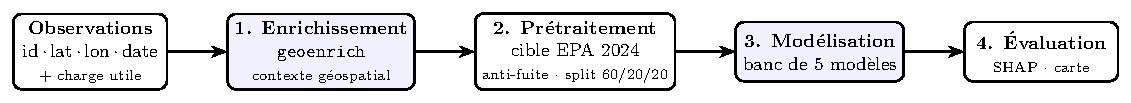
\includegraphics[width=0.92\linewidth]{Chap3/images/latex/schema1.pdf}
    \caption{Vue d'ensemble du pipeline, de l'observation ponctuelle \`a l'\'evaluation interpr\'et\'ee.}
    \label{fig:schema1}
\end{figure}

Cette lin\'earit\'e apparente masque une distinction structurante, introduite d\`es la premi\`ere \'etape et reprise dans tout le travail~: la s\'eparation entre la \emph{charge utile} (ce que l'on mesure et cherche \`a pr\'edire) et le \emph{contexte g\'eographique} (o\`u et quand la mesure a \'et\'e faite). La figure~\ref{fig:schema1bis} d\'etaille l'architecture interne de chaque \'etape.

\begin{figure}[H]
    \centering
    
\includegraphics[width=0.92\linewidth]{Chap3/images/mermaid/schema1bis.png}
    \caption{Architecture interne des \'etapes~: enrichissement (\texttt{geoenrich}), pr\'etraitement (cible EPA 2024, anti-fuite, d\'ecoupage) et mod\'elisation (banc de cinq mod\`eles).}
    \label{fig:schema1bis}
\end{figure}

\mySubSection{Du jeu d'observations au dataset enrichi}{}
\label{sec:contrib-enrichissement-principe}

L'enrichissement repose sur une id\'ee directrice~: tout le contexte g\'eographique d'une observation se d\'eduit de son \emph{o\`u} et de son \emph{quand}, ind\'ependamment de la nature de ce qui est mesur\'e. Un op\'erateur qui calcule la distance au site de contamination le plus proche, ou qui rattache un point \`a son sous-bassin hydrog\'eologique, n'a pas besoin de savoir s'il manipule une mesure de PFAS, de nitrate ou de m\'etaux~: il n'utilise que les coordonn\'ees et la date. La charge utile est transport\'ee sans jamais \^etre lue.

Cette s\'eparation r\'eduit le contrat d'entr\'ee \`a quatre champs canoniques (identifiant, latitude, longitude, date), auxquels n'importe quel jeu d'observations peut \^etre ramen\'e, le reste des colonnes \'etant consid\'er\'e comme charge utile ignor\'ee. L'enrichissement devient alors une op\'eration g\'en\'erique, applicable au-del\`a du cas PFAS qui lui a servi d'instanciation. Sur le dataset californien, cette \'etape attache aux mesures un large \'eventail de variables de contexte (proximit\'e et densit\'e de sites de contamination, propri\'et\'es des sols, variables hydrog\'eologiques, sous-bassins), dont la validit\'e a \'et\'e contr\^ol\'ee par comparaison avec le pipeline initial du projet.

\mySubSection{De l'enrichissement \`a la pr\'ediction}{}
\label{sec:contrib-enrichissement-prediction}
Le dataset enrichi sert de socle commun \`a tous les mod\`eles, ce qui garantit une comparaison \'equitable. Sur ce socle, deux familles de mod\`eles cohabitent. Les mod\`eles tabulaires (for\^et al\'eatoire, gradient boosting) traitent chaque observation comme un vecteur de variables ind\'ependant des autres. Le mod\`ele relationnel (transformeur de graphe h\'et\'erog\`ene) exploite au contraire la structure~: il relie les forages entre eux et \`a des entit\'es partag\'ees (sites de contamination, sous-bassins, voisinages spatiaux) de sorte que des points proches d'une m\^eme source \'echangent de l'information.
Deux mod\`eles hybrides compl\`etent le banc, en combinant les repr\'esentations apprises par le graphe avec les variables tabulaires.

\mySubSection{Principes directeurs}{}
\label{sec:contrib-principes}

Trois principes traversent l'ensemble de la contribution. Le premier est la r\'eutilisabilit\'e de l'outil~: l'enrichissement est con\c{c}u comme un composant g\'en\'erique, le moteur ne contenant aucune r\'ef\'erence au cas PFAS, les sp\'ecificit\'es r\'egionales \'etant rel\'egu\'ees dans une configuration externe rempla\c{c}able sans toucher au code. Le deuxi\`eme est la rigueur de l'\'evaluation~: le dispositif central contre la m\'emorisation g\'eographique est le retrait de la localisation des variables d'entr\'ee, combin\'e \`a sa structuration dans la topologie du graphe relationnel. Le troisi\`eme est l'interpr\'etabilit\'e comme exigence transversale~: chaque mod\`ele est accompagn\'e d'analyses d'importance des variables et d'explications locales, la lisibilit\'e \'etant trait\'ee comme un livrable \`a part enti\`ere dans un contexte environnemental o\`u les pr\'edictions orientent des d\'ecisions de surveillance.


% =========================================================
\mySection{\texttt{geoenrich}~: un moteur d'enrichissement g\'eospatial g\'en\'erique}{}
\label{sec:geoenrich}
% =========================================================

La premi\`ere contribution est un outil~: \texttt{geoenrich}\footnote{D\'ep\^ot public~: \url{https://github.com/dnwiloic/geoenrich}}. Il produit, \`a partir d'un jeu d'observations ponctuelles respectant un contrat d'entr\'ee minimal, un dataset riche en variables contextuelles via une biblioth\`eque d'op\'erateurs enfichables. Le dataset PFAS californien en est la premi\`ere instanciation et non une d\'ependance.

\mySubSection{Motivation}{}
\label{sec:geoenrich-motivation}


La plupart des jeux de donn\'ees consacr\'es aux PFAS pr\'esentent un nombre limit\'e de caract\'eristiques. Ils se limitent g\'en\'eralement aux informations relatives aux puits (localisation, cote ou profondeur), \`a la date de pr\'el\`evement ainsi qu'aux r\'esultats des analyses de laboratoire. Or, la litt\'erature a montr\'e que les informations contextuelles, telles que la proximit\'e et la densit\'e des sites potentiels de contamination, les propri\'et\'es des sols, les variables hydrog\'eologiques ou encore les sous-bassins versants, jouent un r\^ole essentiel dans la pr\'ediction des risques li\'es aux PFAS \`a l'aide de m\'ethodes d'intelligence artificielle~\cite{dong2024pfas,guelfo2021pfas}. L'objectif de \texttt{geoenrich} est donc d'enrichir automatiquement ces jeux de donn\'ees en leur ajoutant des caract\'eristiques environnementales pertinentes, d\'eriv\'ees de la localisation des puits et de la date de pr\'el\`evement, afin d'am\'eliorer les performances des mod\`eles de pr\'ediction.
% Le code initial du projet illustrait le travers des scripts ad hoc~: la logique de jointure tenait dans un module unique de pr\`es de mille lignes, o\`u la m\'ecanique g\'en\'erique d'appariement spatial et temporel se trouvait m\^el\'ee aux particularit\'es du cas PFAS (noms de colonnes propres au programme de surveillance, chemins de couches sp\'ecifiques, r\`egles m\'etier li\'ees au polluant). Un tel code n'est ni testable isol\'ement, ni r\'eutilisable~: changer de polluant ou de r\'egion imposerait de le r\'e\'ecrire. L'objectif de \texttt{geoenrich} est de transformer cette logique monolithique en un composant r\'eutilisable, par une s\'eparation stricte entre le \emph{quoi} (la mesure \'etudi\'ee, simple charge utile transport\'ee) et le \emph{o\`u/quand} (les cl\'es de jointure universelles que sont la position et la date).

\mySubSection{Contrat d'entr\'ee}{}
\label{sec:geoenrich-contrat}

Le contrat d'entr\'ee est l'interface minimale que tout jeu d'observations doit satisfaire pour \^etre enrichi. Il se r\'eduit \`a quatre champs canoniques~: un identifiant de point, une latitude et une longitude en WGS84 (cl\'es de jointure spatiale), et une date (cl\'e de jointure temporelle). Seules la latitude et la longitude sont strictement obligatoires~; l'identifiant est g\'en\'er\'e \`a d\'efaut, et la date n'est requise que si des op\'erateurs temporels sont mobilis\'es. Toute autre colonne est consid\'er\'ee comme charge utile et n'est jamais lue par le moteur. Une fonction de mise au contrat renomme les colonnes du jeu source vers ces noms canoniques, puis une \'etape de validation contr\^ole le typage, supprime les lignes sans coordonn\'ees et analyse les dates. C'est cette r\'eduction \`a quatre champs qui rend le moteur agnostique.

\mySubSection{Architecture en trois couches}{}
\label{sec:geoenrich-architecture}

L'architecture de \texttt{geoenrich} repose sur trois couches strictement s\'epar\'ees, dont la g\'en\'ericit\'e d\'ecro\^it \`a mesure que l'on descend vers le cas concret (figure~\ref{fig:schema2}). La \textbf{couche contrat}, sup\'erieure, est enti\`erement agnostique~: elle ne conna\^it que les quatre cl\'es canoniques et ignore la charge utile. La \textbf{couche op\'erateurs}, interm\'ediaire, rassemble les op\'erateurs d'enrichissement, g\'en\'eriques mais param\'etrables, qui reposent sur deux primitives de jointure seulement~: une primitive spatiale fond\'ee sur un arbre k-d en distance grand-cercle (point source le plus proche, sources dans un rayon, polygone contenant un point) et une primitive temporelle par appariement par ant\'eriorit\'e par entit\'e, avec repli spatial lorsque l'appariement direct \'echoue. La couche configuration, inf\'erieure, est la seule \`a porter le contexte particulier d'une r\'egion~: un fichier YAML d\'eclare la racine des donn\'ees de r\'ef\'erence et la liste ordonn\'ee des op\'erateurs, chacun pointant vers ses couches locales. Un registre interne associe chaque type d'op\'erateur \`a sa classe d'impl\'ementation, de sorte qu'ajouter un op\'erateur ne demande qu'une ligne de configuration, sans modifier le code.

\begin{figure}[H]
    \centering
    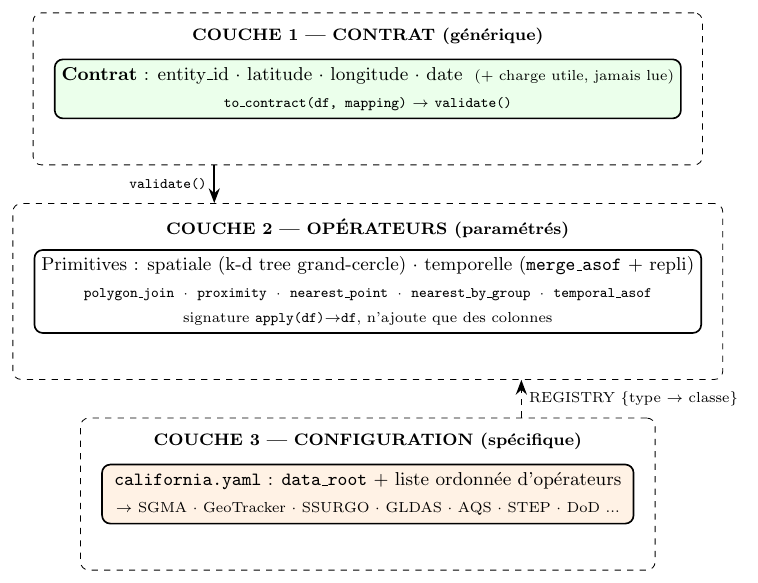
\includegraphics[width=0.88\linewidth]{Chap3/images/latex/schema2.png}
    \caption{Les trois couches de \texttt{geoenrich}~: contrat agnostique, op\'erateurs param\'etr\'es (primitives spatiale et temporelle), configuration sp\'ecifique \`a la r\'egion.}
    \label{fig:schema2}
\end{figure}

\mySubSection{Biblioth\`eque d'op\'erateurs}{}
\label{sec:geoenrich-operateurs}

La biblioth\`eque compte cinq familles d'op\'erateurs, chacune r\'epondant \`a un motif de jointure r\'ecurrent~: \texttt{polygon\_join} rattache un point aux attributs du polygone qui le contient (par exemple le sous-bassin hydrog\'eologique d'un forage)~; \texttt{proximity} calcule la distance au site le plus proche, son type et le nombre de sites dans une s\'erie de rayons~; \texttt{nearest\_point} r\'ecup\`ere les valeurs du point source le plus proche, en version statique ou index\'ee par ann\'ee et par mois~; \texttt{nearest\_by\_group} traite les sources au format long en retrouvant, pour chaque code de variable, le moniteur le plus proche~; \texttt{temporal\_asof} r\'ealise l'appariement temporel par entit\'e avec repli spatial. Ces op\'erateurs partagent quatre propri\'et\'es qui font la robustesse du moteur~: ils sont composables, optionnels (un op\'erateur dont la source est absente est ignor\'e sans interrompre le traitement), idempotents sur le contrat (ils n'ajoutent que des colonnes) et ind\'ependants de la charge utile.

\mySubSection{Entr\'ees, sorties et instanciation californienne}{}
\label{sec:geoenrich-io}

En entr\'ee, \texttt{geoenrich} accepte des observations ponctuelles aux formats CSV, Parquet ou GeoJSON, ramen\'ees au contrat par leur mapping. La sortie est le m\^eme jeu, augment\'e des colonnes produites par chaque op\'erateur et accompagn\'e d'un dictionnaire de donn\'ees d\'ecrivant les variables g\'en\'er\'ees. L'outil s'utilise comme biblioth\`eque Python et en ligne de commande. Pour le cas californien, la configuration instancie neuf op\'erateurs mobilisant autant de couches de r\'ef\'erence~: sous-bassins hydrog\'eologiques, sites de contamination, stations d'\'epuration, sites f\'ed\'eraux li\'es \`a la d\'efense (source majeure de PFAS par les mousses anti-incendie, section~\ref{sec:pfas-usages-sources}), d\'echarges, propri\'et\'es des sols, variables hydrologiques mensuelles, qualit\'e de l'air et co-contaminants par appariement temporel, auxquels s'ajoutent l'occupation du sol et la topographie extraites par \'echantillonnage raster. \`A partir des seules coordonn\'ees et dates, l'ensemble produit un contexte environnemental riche pour chaque mesure.

\mySubSection{Le jeu de donn\'ees d'application~: de la base GAMA au dataset enrichi}{}
\label{sec:geoenrich-dataset}

L'instanciation californienne de \texttt{geoenrich} produit le jeu de donn\'ees qui sert \`a entra\^iner et \'evaluer les mod\`eles de la section~\ref{sec:contrib-modeles}. Cette sous-section en d\'ecrit l'origine, la base d'observations brutes, puis le jeu enrichi et son remplissage.

\mySubSubSection{Origine et reconstruction de la base}{}
\label{sec:geoenrich-dataset-origine}

Le dataset qui sert de base pour l'enrichissement a \'et\'e constitu\'e \`a partir de deux fichiers bruts du programme GAMA, \texttt{gama\_allwells}\footnote{\url{https://data.ca.gov/dataset/ground-water-water-quality-results/resource/805e6762-1b82-48d9-b68f-5d79cca06ace}} et \texttt{pfas}\footnote{\url{https://data.ca.gov/dataset/ground-water-water-quality-results/resource/c7cd50a2-2a68-44a1-8d40-4e767f363964}}. La fusion consiste \`a ramener toutes les mesures de contaminant d'un puits ainsi que la date de pr\'el\`evement sur une m\^eme ligne contenant \'egalement les coordonn\'ees g\'eographiques du puits. Cette op\'eration a pour but de respecter le contrat d'entr\'ee de \texttt{geoenrich}. Le dataset obtenu, nomm\'e \texttt{wells\_pfas\_cleaned}, couvre 46\,338 pr\'el\`evements sur environ 11\,300 puits, r\'epartis sur les 58 comt\'es de l'\'Etat, entre avril 2016 et janvier 2026, un p\'erim\`etre plus large et plus r\'ecent que celui de Dong et al.~\cite{dong2024pfas}. Chaque pr\'el\`evement porte une cl\'e d'identit\'e minimale et ses mesures comme indiqu\'e dans le tableau~\ref{tab:base-brute}.

\begin{table}[h!]
    \centering
    \caption{Familles de colonnes de la base d'observations brutes (avant enrichissement).}
    \label{tab:base-brute}
    \small
    \begin{tabular}{l p{5.3cm} p{4.6cm}}
        \hline
        Cat\'egorie & Colonnes (exemples) & R\^ole \\
        \hline
        Identit\'e & \texttt{gm\_well\_id}, \texttt{gm\_dataset\_name}, \texttt{gm\_well\_category} & puits, programme source (6), type de puits (5) \\
        Localisation & \texttt{latitude}, \texttt{longitude}, \texttt{county}, \texttt{regional\_board} & cl\'es spatiales, d\'ecoupage administratif \\
        Temps & \texttt{collection\_date} & date du pr\'el\`evement (2\,069 dates distinctes) \\
        Mesures PFAS & 32 colonnes \texttt{*\_ngL} & concentrations par esp\`ece (PFOA, PFOS, PFHxS, PFBS, etc.) \\
        D\'etection & 62 colonnes \texttt{*\_detected}, \texttt{label\_*} & indicateurs de d\'etection par esp\`ece \\
        \hline
    \end{tabular}
\end{table}

La caract\'eristique notable de cette base est que les concentrations elles-m\^emes sont tr\`es lacunaires~: toutes les esp\`eces ne sont pas dos\'ees \`a chaque pr\'el\`evement, si bien que la majorit\'e des 32 colonnes \texttt{*\_ngL} d\'epasse 40~\% de valeurs manquantes. Ces colonnes d\'efinissent la cible et sont \'ecart\'ees comme fuite (section~\ref{sec:contrib-pretraitement})~; leur lacune n'affecte donc pas la mod\'elisation. Hors PFAS, la base brute n'apporte qu'un contexte tr\`es limit\'e, d'o\`u le recours \`a l'enrichissement.

\mySubSubSection{Le jeu enrichi~: structure et familles de colonnes}{}
\label{sec:geoenrich-dataset-enrichi}

Apr\`es passage par \texttt{geoenrich}, le jeu compte 217 colonnes (131 r\'eelles, 41 enti\`eres, 31 bool\'eennes, 13 textuelles, 1 date) pour les m\^emes 46\,338 pr\'el\`evements. \`A la base s'ajoutent les familles de variables contextuelles r\'esum\'ees au tableau~\ref{tab:familles-enrichies}.

\begin{table}[h!]
    \centering
    \caption{Familles de variables contextuelles ajout\'ees par \texttt{geoenrich} (nombre de colonnes et taux moyen de valeurs manquantes).}
    \label{tab:familles-enrichies}
    \small
    \begin{tabular}{p{4.2cm} p{6.2cm} c c}
        \hline
        Famille (source) & Pr\'efixe / colonnes & Nb & NA \% moyen \\
        \hline
        Sites de contamination GeoTracker & \texttt{dist\_geotracker\_km}, \texttt{n\_geotracker\_within\_\{1,3,10,50\}km}, \texttt{nearest\_geotracker\_type} & 6 & 0 \\
        Co-contaminants (GAMA) & \texttt{cocontam\_*} & 44 & 16,5 \\
        Sol (SSURGO) & \texttt{soil\_*} & 26 & 20,5 \\
        Qualit\'e de l'air (AQS) & \texttt{aqs\_*} & 8 & 9,9 \\
        Hydrom\'et\'eorologie (GLDAS) & \texttt{rainfall\_mm\_month}, \texttt{et\_mm\_month}, \texttt{runoff\_mm}, \texttt{temp\_c}, \texttt{snowpack\_mm}, \texttt{root\_zone\_moist\_kg\_m2} & 7 & $\sim$4 \\
        Bassins hydrog\'eologiques (SGMA) & \texttt{sgma\_*} & 3 & 6,1 \\
        Niveaux de nappe et gradient (DWR) & \texttt{depth\_to\_water\_m}, \texttt{dist\_nearest\_gwl\_km}, \texttt{hydr\_grad\_mag\_permil}, \texttt{flow\_dir\_sin/cos} & 6 & $\sim$0 \\
        Topographie (USGS 3DEP) & \texttt{elevation\_m} & 1 & 10,4 \\
        Occupation du sol (NLCD) & \texttt{dev\_intensity}, \texttt{lc\_developed} & 2 & 0 \\
        G\'eom\'etrie de forage & \texttt{well\_depth\_ft}, \texttt{screen\_mid\_ft}, \texttt{screen\_length\_ft}, \texttt{depth\_eff\_ft} & 4 & 49 \`a 95 \\
        Indicateurs d'absence (ing\'enierie) & \texttt{depth\_missing}, \texttt{topo\_missing} & 2 & 0 \\
        \hline
    \end{tabular}
\end{table}

Ces familles couvrent les hypoth\`eses m\'ecanistes de la contamination~: proximit\'e des sources, nature du sol, hydrologie, co-pollution, contexte hydrog\'eologique.

\mySubSubSection{Remplissage des colonnes}{}
\label{sec:geoenrich-dataset-remplissage}

Le profil de compl\'etude du jeu enrichi est globalement favorable~: sur les 217 colonnes, 88 sont renseign\'ees \`a 100~\% et 80 le sont \`a plus de 90~\%. Les variables de contexte ajout\'ees par l'enrichissement spatial (proximit\'e GeoTracker, occupation du sol, niveaux de nappe) sont presque toujours compl\`etes, parce qu'elles r\'esultent d'une jointure g\'eographique qui aboutit pour tout point situ\'e dans l'emprise des couches de r\'ef\'erence.

Trente et une colonnes d\'epassent 40~\% de valeurs manquantes. Leur examen est rassurant~: 17 sont des concentrations \texttt{*\_ngL}, d\'ej\`a \'elimin\'ees comme fuite, et les 14 restantes se r\'epartissent entre la g\'eom\'etrie de forage (\texttt{well\_depth\_ft} \`a 95~\%, \texttt{screen\_*} et \texttt{depth\_eff\_*} autour de 50~\%, rarement document\'es dans GAMA), la granulom\'etrie fine du sol et quelques co-contaminants rares. Le signal hydrog\'eologique que portait la g\'eom\'etrie de forage est partiellement r\'ecup\'er\'e par des proxys mieux renseign\'es et conserv\'es, la profondeur de la nappe (\texttt{depth\_to\_water\_m}), la distance au point de mesure pi\'ezom\'etrique (\texttt{dist\_nearest\_gwl\_km}) et le gradient hydraulique (\texttt{hydr\_grad\_mag\_permil}), tous complets. Enfin, des indicateurs binaires d'absence (\texttt{depth\_missing}, \texttt{topo\_missing}) encodent explicitement la lacune sans inventer de valeur. C'est ce jeu enrichi, une fois \'ecart\'ees les colonnes de fuite, les variables trop lacunaires et la localisation, qui alimente les mod\`eles de la section~\ref{sec:contrib-modeles}.


% =========================================================
\mySection{Mod\`eles de pr\'ediction de la contamination}{}
\label{sec:contrib-modeles}
% =========================================================

La seconde contribution est un banc de cinq mod\`eles pr\'edisant, pour chaque pr\'el\`evement, le risque de d\'epassement du seuil r\'eglementaire EPA 2024. Tous partagent le m\^eme dataset enrichi, la m\^eme cible et le m\^eme d\'ecoupage, ce qui rend leur comparaison \'equitable (figure~\ref{fig:schema3}). Le fil directeur est la question de recherche pos\'ee en introduction (section~\ref{sec:contrib-intro})~: le signal spatial doit-il \^etre m\'emoris\'e comme variable ou structur\'e dans la topologie d'un graphe~? La r\'eponse op\'erationnelle est le retrait de la localisation de toutes les variables, celle-ci n'intervenant que dans la construction du graphe.

\begin{figure}[H]
    \centering
    
\includegraphics[width=0.92\linewidth]{Chap3/images/mermaid/schema3.png}
    \caption{Le banc des cinq mod\`eles sur socle commun (dataset enrichi, d\'ecoupage 60/20/20) et les d\'ependances des mod\`eles hybrides (fusion par embeddings, stacking).}
    \label{fig:schema3}
\end{figure}

On observe que les cinq mod\`eles partent du m\^eme dataset enrichi et du m\^eme d\'ecoupage 60/20/20, ce qui garantit une comparaison \'equitable~: les \'ecarts de performance mesur\'es plus loin tiennent au mod\`ele et non aux donn\'ees. La figure distingue aussi deux niveaux. Les deux arbres de r\'ef\'erence et le HGT s'entra\^inent directement sur le socle commun, tandis que les deux mod\`eles hybrides en d\'ependent~: la fusion par embeddings r\'eutilise les repr\'esentations apprises par le HGT, et le stacking combine les pr\'edictions des trois mod\`eles de base. Ces fl\`eches de d\'ependance expliquent l'ordre dans lequel les mod\`eles sont pr\'esent\'es et entra\^in\'es par la suite.

\mySubSection{Donn\'ees et cible}{}
\label{sec:contrib-donnees}

L'\'etude porte sur 46\,338 pr\'el\`evements d'eaux souterraines californiennes~\cite{dong2024pfas}, enrichis par \texttt{geoenrich} (section~\ref{sec:geoenrich}) puis ramen\'es \`a 97 variables explicatives apr\`es nettoyage (94 num\'eriques et 3 cat\'egorielles). Ces variables d\'ecrivent le contexte du forage (proximit\'e et densit\'e de sites de contamination, sol, hydrologie, qualit\'e de l'air, co-contaminants), \`a l'exclusion de toute concentration en PFAS, conform\'ement au mode pr\'edictif.

\paragraph{Construction de la cible}{}
\label{sec:contrib-cible}

La cible est binaire et reproduit la r\`egle de d\'epassement du r\`eglement EPA 2024 NPDWR (section~\ref{sec:pfas-reglementation})~\cite{epa2023npdwr}. Deux crit\`eres ind\'ependants peuvent la d\'eclencher, correspondant aux deux volets du r\`eglement.

Le \textbf{crit\`ere individuel} vaut 1 d\`es qu'une concentration mesur\'ee d\'epasse son MCL, fix\'e \`a 4~ng/L pour le PFOA et le PFOS, et \`a 10~ng/L pour le PFNA, le PFHxS et le HFPO-DA. Le \textbf{crit\`ere de m\'elange} s'appuie sur l'indice de risque (HI)~: il est d\'eclench\'e lorsque $\mathrm{HI} > 1$, c'est-\`a-dire lorsque les effets cumul\'es des compos\'es d\'epassent le niveau jug\'e admissible. Le tableau~\ref{tab:epa2024-seuils} r\'esume les six compos\'es couverts et les valeurs num\'eriques utilis\'ees.

\begin{table}[H]
    \centering
    \caption{Seuils EPA 2024 NPDWR impl\'ement\'es dans la construction de la cible.}
    \label{tab:epa2024-seuils}
    \begin{tabular}{lllcc}
        \hline
        Compos\'e & Sigle & Classe & MCL (ng/L) & $\mathrm{VR}_i$ HI (ng/L) \\
        \hline
        Acide perfluoroocta\-no\"ique       & PFOA    & PFCA & 4   & N.A.  \\
        Sulfonate de perfluorooctane        & PFOS    & PFSA & 4   & N.A.  \\
        Acide perfluorononano\"ique         & PFNA    & PFCA & 10  & 10   \\
        Acide perfluorohexane sulfonique    & PFHxS   & PFSA & 10  & 10   \\
        Acide dim\'erique HFPO (GenX)       & HFPO-DA & N.A. & 10  & 10   \\
        Acide perfluorobutane sulfonique    & PFBS    & PFSA & N.A. & 2000 \\
        \hline
    \end{tabular}
\end{table}

Le HI est calcul\'e sur les quatre compos\'es pour lesquels l'EPA fournit une valeur sanitaire de r\'ef\'erence $\mathrm{VR}_i$~:
\[
    \mathrm{HI}
    = \frac{C_{\mathrm{PFNA}}}{10}
    + \frac{C_{\mathrm{PFHxS}}}{10}
    + \frac{C_{\mathrm{HFPO\text{-}DA}}}{10}
    + \frac{C_{\mathrm{PFBS}}}{2000}
\]
o\`u toutes les concentrations $C_i$ sont exprim\'ees en ng/L. On notera que le PFNA, le PFHxS et le HFPO-DA figurent dans les deux crit\`eres~: d\'epasser 10~ng/L pour l'un de ces compos\'es d\'eclenche simultan\'ement le MCL individuel et alourdit le HI.

Un pr\'el\`evement est \'etiquet\'e \`a risque (cible $= 1$) d\`es qu'au moins l'un des deux crit\`eres est franchi, et conforme (cible $= 0$) sinon. Le calcul part des concentrations brutes~; les valeurs manquantes sont assimil\'ees \`a des non-d\'etections et contribuent donc pour z\'ero aux deux crit\`eres.

Le jeu obtenu est presque \'equilibr\'e~: 21\,154 pr\'el\`evements positifs (45,65~\% de l'\'echantillon), ce qui \'evite de recourir \`a un r\'e\'echantillonnage artificiel. La figure~\ref{fig:class-distribution} pr\'esente cette distribution.

\begin{figure}[H]
    \centering
    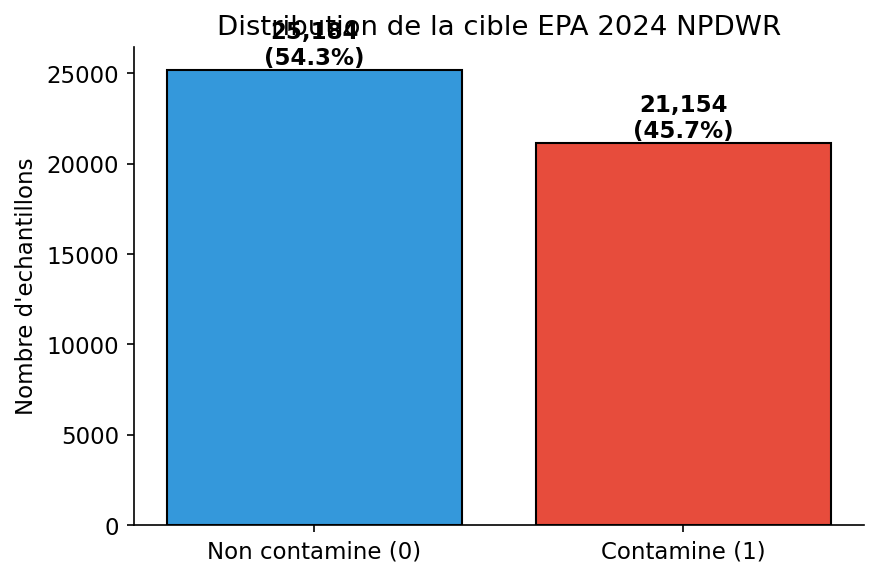
\includegraphics[width=0.6\linewidth]{Chap3/images/figures/fig01_class_distribution.png}
    \caption{Distribution des classes de la cible EPA 2024 sur le jeu complet.}
    \label{fig:class-distribution}
\end{figure}
On constate que les deux classes sont presque \'equilibr\'ees, ce qui justifie d'\'evaluer les mod\`eles sans correction de d\'es\'equilibre et de privil\'egier des m\'etriques de discrimination plut\^ot qu'une simple exactitude.

\mySubSection{Pr\'etraitement et ing\'enierie des variables}{}
\label{sec:contrib-pretraitement}

Le pr\'etraitement est appliqu\'e de mani\`ere identique aux cinq mod\`eles, \`a partir du seul jeu d'entra\^inement pour \'eviter toute fuite. Il combine quatre d\'ecisions. La premi\`ere est l'\textbf{\'elimination des fuites}~: la cible \'etant une fonction d\'eterministe des concentrations, toute variable qui r\'eexprime cette information est retir\'ee (concentrations, indicateurs de d\'etection, ainsi que des colonnes proxy comme le nom du programme de surveillance, corr\'el\'e au protocole d'\'echantillonnage). La deuxi\`eme est un \textbf{seuil de valeurs manquantes}~: toute colonne renseign\'ee \`a moins de 60~\% est \'ecart\'ee, l'imputation au-del\`a inventant la majorit\'e de la colonne. La troisi\`eme, la plus structurante, est le retrait de la localisation des variables~: latitude, longitude, comt\'e et d\'ecoupages administratifs sont exclus des variables de chaque mod\`ele, car la contamination PFAS \'etant fortement auto-corr\'el\'ee dans l'espace, les conserver laisserait les mod\`eles m\'emoriser la g\'eographie au lieu d'apprendre des m\'ecanismes~; les coordonn\'ees ne sont conserv\'ees que pour b\^atir le graphe. La quatri\`eme est le codage~: imputation m\'ediane des num\'eriques, cat\'egorie \texttt{Unknown} et encodage ordinal des cat\'egorielles, avec une standardisation suppl\'ementaire pour le r\'eseau de neurones. Le jeu est ensuite s\'epar\'e en train, validation et test (60/20/20) de fa\c{c}on stratifi\'ee, soit 27\,802, 9\,268 et 9\,268 pr\'el\`evements, ce d\'ecoupage \'etant partag\'e par les cinq mod\`eles.

\mySubSection{Mod\`eles tabulaires de r\'ef\'erence}{}
\label{sec:contrib-tabulaires}

Deux mod\`eles d'arbres servent de r\'ef\'erence, car ils repr\'esentent l'\'etat de l'art pratique sur donn\'ees tabulaires et fixent le niveau de performance \`a atteindre. La \textbf{for\^et al\'eatoire} et \textbf{XGBoost}, introduits au chapitre~\ref{chap:generalites} (sections~\ref{sec:bagging} et~\ref{sec:boosting}), traitent chaque pr\'el\`evement comme un vecteur de variables ind\'ependant des autres. Leurs hyperparam\`etres sont optimis\'es par Optuna~; les espaces de recherche et les valeurs retenues sont d\'etaill\'es en annexe~\ref{ann:hyperparams}.

La figure~\ref{fig:rf-lc} montre la courbe d'apprentissage de la for\^et al\'eatoire~: l'erreur \emph{out-of-bag} (OOB, axe gauche) est trac\'ee contre l'AUC sur la validation (axe droit) en fonction du nombre d'arbres construits.

\begin{figure}[H]
    \centering
    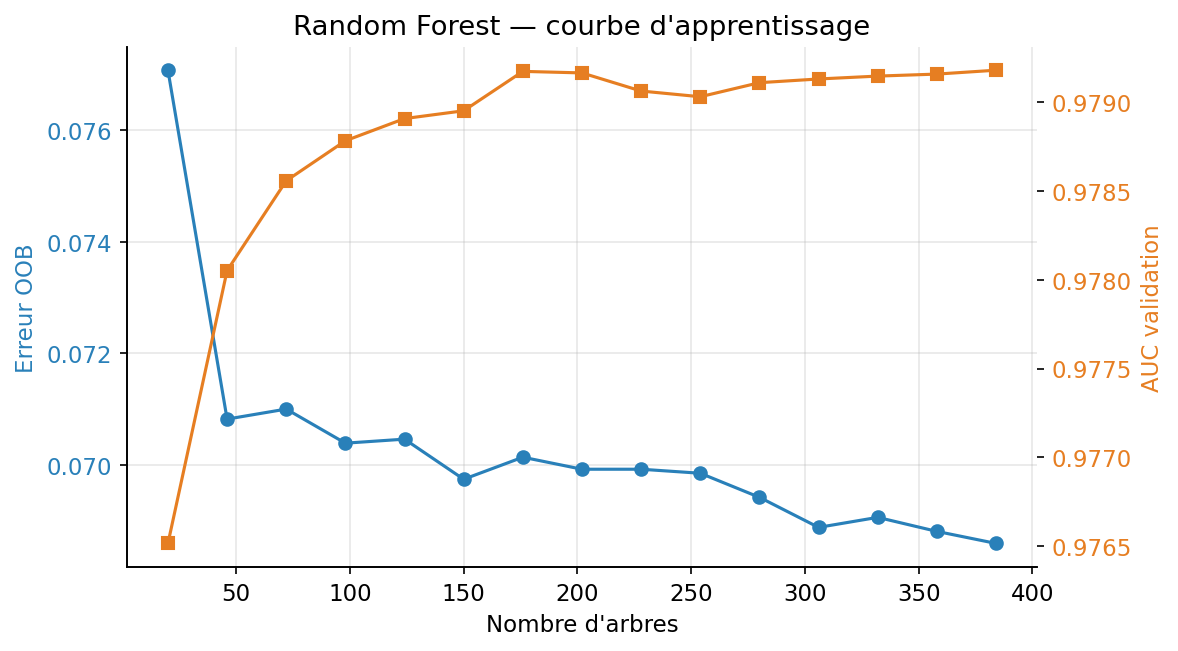
\includegraphics[width=0.82\linewidth]{Chap3/images/figures/fig04_rf_learning_curve.png}
    \caption{For\^et al\'eatoire~: erreur OOB (bleu, axe gauche) et AUC de validation (orange, axe droit) selon le nombre d'arbres.}
    \label{fig:rf-lc}
\end{figure}

On observe que l'erreur OOB d\'ecro\^it rapidement puis se stabilise autour de 0,069 (score OOB = 0,931), tandis que l'AUC de validation progresse dans la m\^eme direction et atteint un plateau~; la convergence de ces deux indicateurs ind\'ependants confirme que le mod\`ele g\'en\'eralise sans surapprentissage.

La figure~\ref{fig:xgb-lc} pr\'esente la courbe d'apprentissage de XGBoost~: la perte sur l'entra\^inement et l'AUC sur la validation sont suivies \`a chaque it\'eration de boosting, un arr\^et anticip\'e (\emph{early stopping}) interrompant l'entra\^inement si la validation ne s'am\'eliore plus pendant 50 it\'erations cons\'ecutives.

\begin{figure}[H]
    \centering
    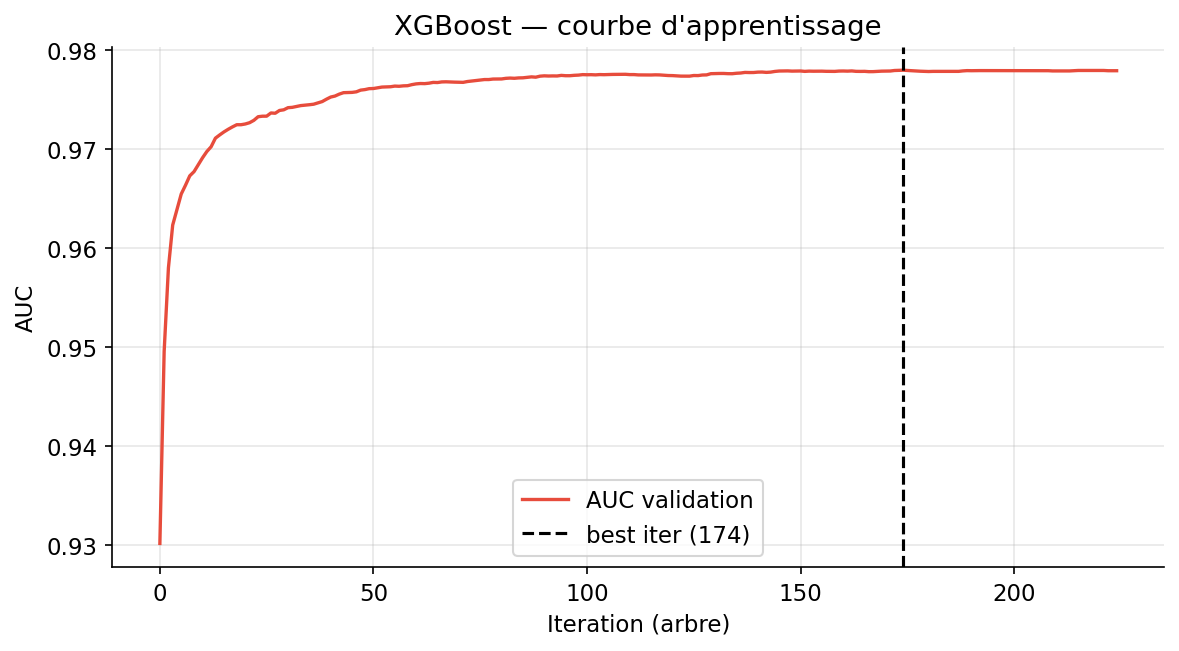
\includegraphics[width=0.82\linewidth]{Chap3/images/figures/fig09_xgb_learning_curve.png}
    \caption{XGBoost~: \'evolution de la perte d'entra\^inement et de l'AUC de validation selon le nombre d'it\'erations de boosting~; la ligne verticale indique l'it\'eration retenue par arr\^et anticip\'e.}
    \label{fig:xgb-lc}
\end{figure}

On observe que la perte d'entra\^inement d\'ecro\^it r\'eguli\`erement tandis que l'AUC de validation se stabilise rapidement~; l'arr\^et anticip\'e s\'electionne l'it\'eration~174 sur les 1\,900 disponibles, ce qui montre que le mod\`ele converge bien avant d'\'epuiser son budget et qu'il n'est pas sous-param\'etr\'e.

\mySubSection{Mod\`ele relationnel~: HGT}{}
\label{sec:contrib-hgt}

Le c\oe ur du second volet est un transformeur de graphe h\'et\'erog\`ene (HGT), dont le principe a \'et\'e pr\'esent\'e \`a la section~\ref{sec:hgt}~; nous en d\'ecrivons ici l'instanciation propre \`a la pr\'ediction PFAS. Le graphe repose sur de v\'eritables entit\'es partag\'ees plut\^ot que sur des attributs recopi\'es (figure~\ref{fig:schema4}). Les n\oe uds \texttt{sample} repr\'esentent les pr\'el\`evements, sans aucune variable de localisation. Trois types de n\oe uds-relais portent le contexte spatial~: les sites de contamination (\texttt{source}), les sous-bassins hydrog\'eologiques (\texttt{subbasin}) et des clusters g\'eographiques obtenus par KMeans (\texttt{geo\_cluster}). Des ar\^etes \texttt{near\_geo} relient directement les pr\'el\`evements \`a leurs plus proches voisins spatiaux. Deux forages proches d'un m\^eme site ou d'un m\^eme sous-bassin \'echangent ainsi de l'information. Pour \'eviter toute fuite, clusters, voisinages et sous-bassins sont construits \`a l'int\'erieur de chaque partition.

\begin{figure}[H]
    \centering
    
\includegraphics[width=0.9\linewidth]{Chap3/images/mermaid/schema4.png}
    \caption{Graphe h\'et\'erog\`ene relationnel~: les n\oe uds \texttt{sample} ne portent aucune variable de localisation~; ils sont reli\'es \`a des entit\'es partag\'ees (\texttt{source}, \texttt{subbasin}, \texttt{geo\_cluster}) et entre eux par des ar\^etes spatiales \texttt{near\_geo}.}
    \label{fig:schema4}
\end{figure}

Le HGT propage l'information le long des ar\^etes par un m\'ecanisme d'attention propre \`a chaque type de relation~: un n\oe ud \texttt{sample} agr\`ege diff\'eremment les messages venus d'un site, d'un sous-bassin ou d'un voisin spatial (figure~\ref{fig:schema5}). Apr\`es plusieurs couches, chaque pr\'el\`evement dispose d'un vecteur de repr\'esentation qui r\'esume son contexte relationnel et alimente un classifieur final. L'entra\^inement s'\'etend sur 300 \'epoques avec optimisation Optuna~; deux techniques d'augmentation r\'egularisent le mod\`ele~: l'ajout de bruit gaussien sur les variables des n\oe uds et le retrait al\'eatoire d'ar\^etes (DropEdge)~; le mod\`ele retenu est celui qui maximise le F1 sur la validation.

\begin{figure}[H]
    \centering
    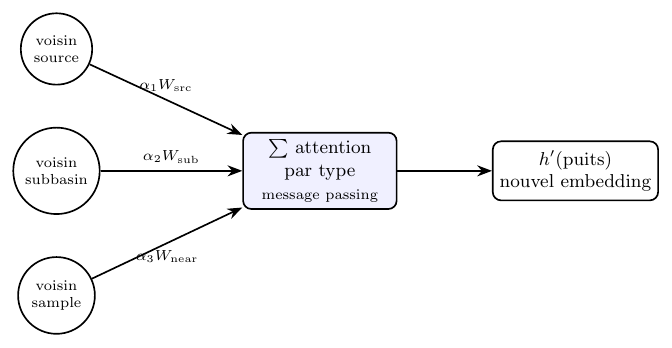
\includegraphics[width=0.9\linewidth]{Chap3/images/latex/schema5.png}
    \caption{M\'ecanisme d'une couche HGT~: passage de message et attention propre \`a chaque type d'ar\^ete, sur le voisinage d'un forage.}
    \label{fig:schema5}
\end{figure}

La figure~\ref{fig:hgt-lc} pr\'esente la courbe d'apprentissage du HGT~: perte d'entra\^inement et F1 de validation sont suivis sur les 300 \'epoques. Optuna a retenu une architecture \`a une seule couche de convolution (\texttt{num\_layers = 1}), ce qui limite la propagation de l'information \`a un saut dans le graphe~: chaque forage agr\`ege uniquement ses voisins directs, sans acc\`es \`a des informations de second rang.

\begin{figure}[H]
    \centering
    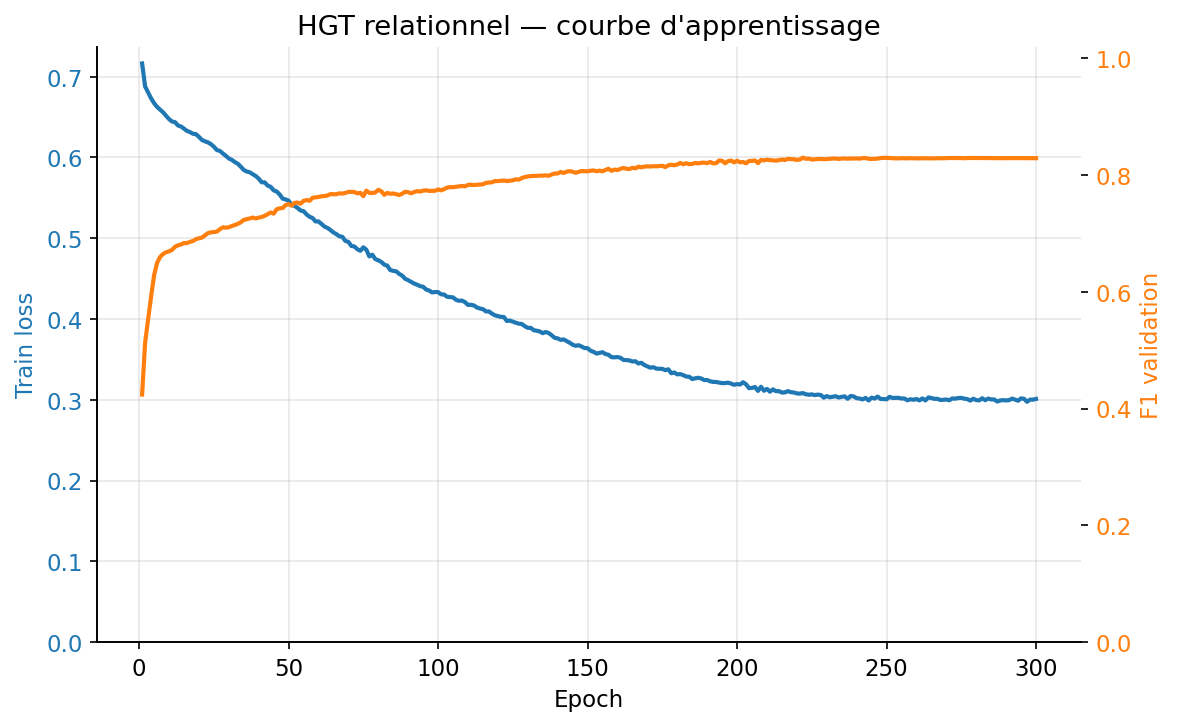
\includegraphics[width=0.82\linewidth]{Chap3/images/figures/fig14_hgt_learning_curve.png}
    \caption{HGT relationnel~: perte d'entra\^inement (axe gauche, bleu) et F1 de validation (axe droit, orange) selon l'\'epoque~; le mod\`ele retenu est celui qui maximise le F1 sur la validation.}
    \label{fig:hgt-lc}
\end{figure}

On observe que la convergence est lente~: le F1 de validation d\'emarre \`a 0,42 \`a la premi\`ere \'epoque et n'atteint 0,78 qu'apr\`es la centaine d'\'epoques. La perte d'entra\^inement d\'ecro\^it r\'eguli\`erement sans diverger, signe que le graphe apprend un signal r\'eel, mais \`a une vitesse et un niveau de performance sensiblement inf\'erieurs \`a ceux des mod\`eles tabulaires.

\mySubSection{Mod\`eles hybrides}{}
\label{sec:contrib-hybrides}

Deux mod\`eles cherchent \`a combiner le meilleur des deux familles.

La \textbf{fusion par embeddings} extrait le vecteur de repr\'esentation (128 dimensions) appris par le HGT pour chaque forage, le compresse par ACP en 2 composantes capturant 97~\% de la variance, puis concat\`ene ces deux composantes aux 97 variables tabulaires. La matrice r\'esultante (99 colonnes) est fournie \`a un XGBoost optimis\'e ind\'ependamment. Ce mod\`ele teste si la repr\'esentation relationnelle du graphe apporte un compl\'ement aux variables de contexte d\'ej\`a pr\'esentes.

Le \textbf{stacking} repose sur un m\'eta-apprentissage en deux \'etapes (section~\ref{sec:stacking}). Les trois mod\`eles de base (RF, XGBoost, HGT) produisent, pour chaque forage, leurs probabilit\'es de d\'epassement~; ces sorties sont compl\'et\'ees par 19 m\'eta-caract\'eristiques~: probabilit\'es brutes, entropies, niveaux de confiance, produits et diff\'erences crois\'es entre mod\`eles, ainsi qu'une composante ACP des embeddings HGT. Un m\'eta-classifieur XGBoost, optimis\'e par Optuna, apprend \`a arbitrer entre les mod\`eles selon la configuration de ces m\'eta-caract\'eristiques.

\mySubSection{Protocole exp\'erimental}{}
\label{sec:contrib-protocole}

L'\'evaluation repose sur des m\'etriques adapt\'ees \`a une cible presque \'equilibr\'ee mais \`a enjeu asym\'etrique~: aire sous la courbe ROC et pr\'ecision moyenne pour le pouvoir de discrimination, rappel et pr\'ecision pour le compromis de d\'ecision, F1 et exactitude \'equilibr\'ee pour une synth\`ese. Chaque mod\`ele est optimis\'e par Optuna sur la validation, et sa robustesse est contr\^ol\'ee par une matrice de confusion. Le dispositif principal contre la m\'emorisation g\'eographique reste le retrait de la localisation des variables (section~\ref{sec:contrib-pretraitement}). La g\'en\'eralisation \`a des r\'egions non vues n'est pas test\'ee dans ce travail~: aucune validation crois\'ee spatiale par blocs n'a \'et\'e conduite, ce point \'etant discut\'e en section~\ref{sec:contrib-discussion}.


% =========================================================
\mySection{R\'esultats, interpr\'etabilit\'e et discussion}{}
\label{sec:contrib-resultats}
% =========================================================

Cette section rapporte les performances des cinq mod\`eles sur le jeu de test (9\,268 pr\'el\`evements, mode pr\'edictif), rend leurs d\'ecisions lisibles aux niveaux global et local, ouvre la bo\^ite noire du graphe, restitue les pr\'edictions sous forme cartographique, puis discute la port\'ee des r\'esultats.

\mySubSection{Performances compar\'ees}{}
\label{sec:contrib-perf}

Le tableau~\ref{tab:comparaison-modeles-chap3} r\'esume les performances sur le test. Les mod\`eles tabulaires dominent nettement~: la for\^et al\'eatoire et XGBoost atteignent une aire sous la courbe ROC proche de 0,98, et le stacking les \'egale sans les d\'epasser. Le HGT relationnel, qui ne re\c{c}oit la g\'eographie que par la structure du graphe, reste en retrait (ROC-AUC 0,906), la fusion se situant entre les deux familles.

\begin{table}[h!]
    \centering
    \caption{Performances compar\'ees des cinq mod\`eles sur le jeu de test (mode pr\'edictif, 9\,268 pr\'el\`evements). Meilleure valeur par colonne en gras.}
    \label{tab:comparaison-modeles-chap3}
    \begin{tabular}{lcccccc}
        \hline
        Mod\`ele & ROC-AUC & AP & Pr\'ecision & Rappel & F1 & Bal. Acc. \\
        \hline
        For\^et al\'eatoire & \textbf{0,979} & \textbf{0,976} & \textbf{0,930} & 0,920 & \textbf{0,925} & \textbf{0,931} \\
        Stacking         & 0,977 & 0,974 & 0,923 & \textbf{0,926} & 0,925 & 0,931 \\
        XGBoost          & 0,977 & 0,974 & 0,922 & 0,923 & 0,923 & 0,929 \\
        Fusion embeddings & 0,960 & 0,954 & 0,886 & 0,887 & 0,887 & 0,896 \\
        HGT relationnel  & 0,906 & 0,886 & 0,823 & 0,828 & 0,825 & 0,839 \\
        \hline
    \end{tabular}
\end{table}

La figure~\ref{fig:roc-pr-all} compl\`ete ce tableau par les courbes ROC et pr\'ecision-rappel des cinq mod\`eles.

\begin{figure}[H]
    \centering
    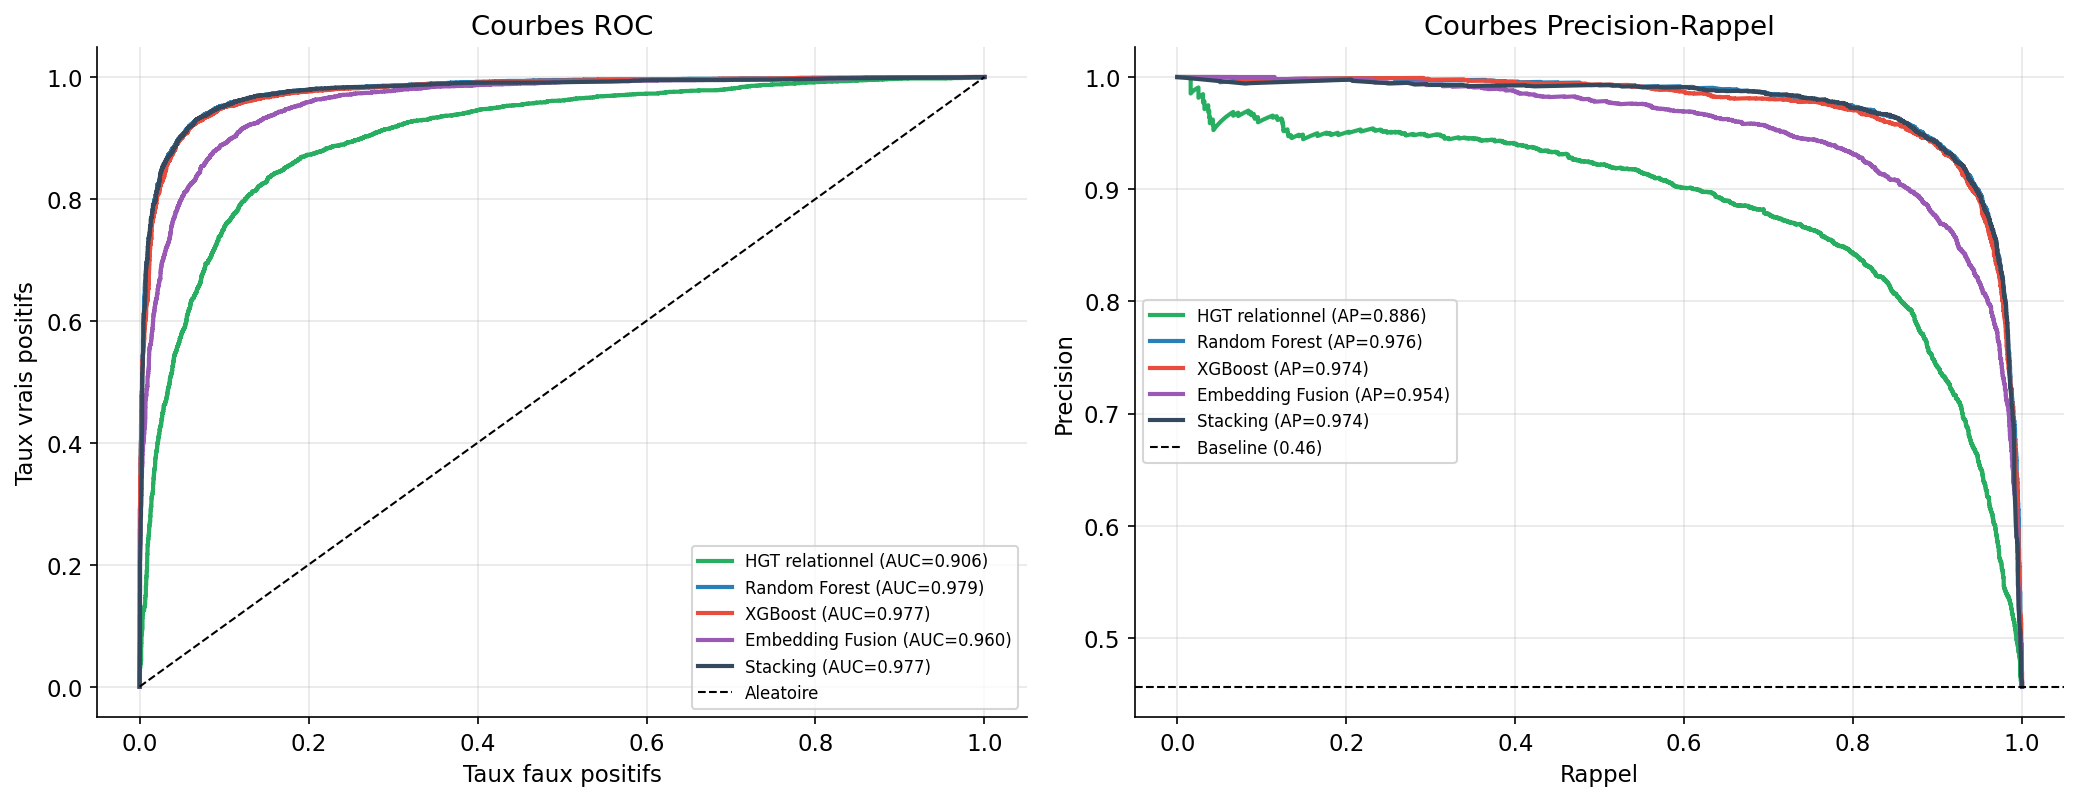
\includegraphics[width=0.95\linewidth]{Chap3/images/figures/fig24_roc_pr_all.png}
    \caption{Courbes ROC et pr\'ecision-rappel des cinq mod\`eles sur le jeu de test (mode pr\'edictif).}
    \label{fig:roc-pr-all}
\end{figure}
On observe que les trois mod\`eles \`a base d'arbres se superposent dans le coin sup\'erieur des deux courbes, tandis que le HGT relationnel forme une courbe nettement plus basse~: structurer la g\'eographie dans un graphe capte un signal r\'eel mais plus pauvre que les variables de contexte. Trois constats se d\'egagent. D'abord, retirer la localisation des variables n'effondre pas les mod\`eles tabulaires, qui restent tr\`es performants en s'appuyant sur les variables issues de \texttt{geoenrich}. Ensuite, structurer la g\'eographie dans un graphe ne suffit pas \`a \'egaler ces variables de contexte. Enfin, les hybrides ne tirent pas profit du relationnel~: la fusion dilue l\'eg\`erement la performance tabulaire et le stacking se contente d'\'egaler la for\^et al\'eatoire, signe d'une faible compl\'ementarit\'e entre les familles. La figure~\ref{fig:dashboard} en donne une vue synth\'etique.

\begin{figure}[H]
    \centering
    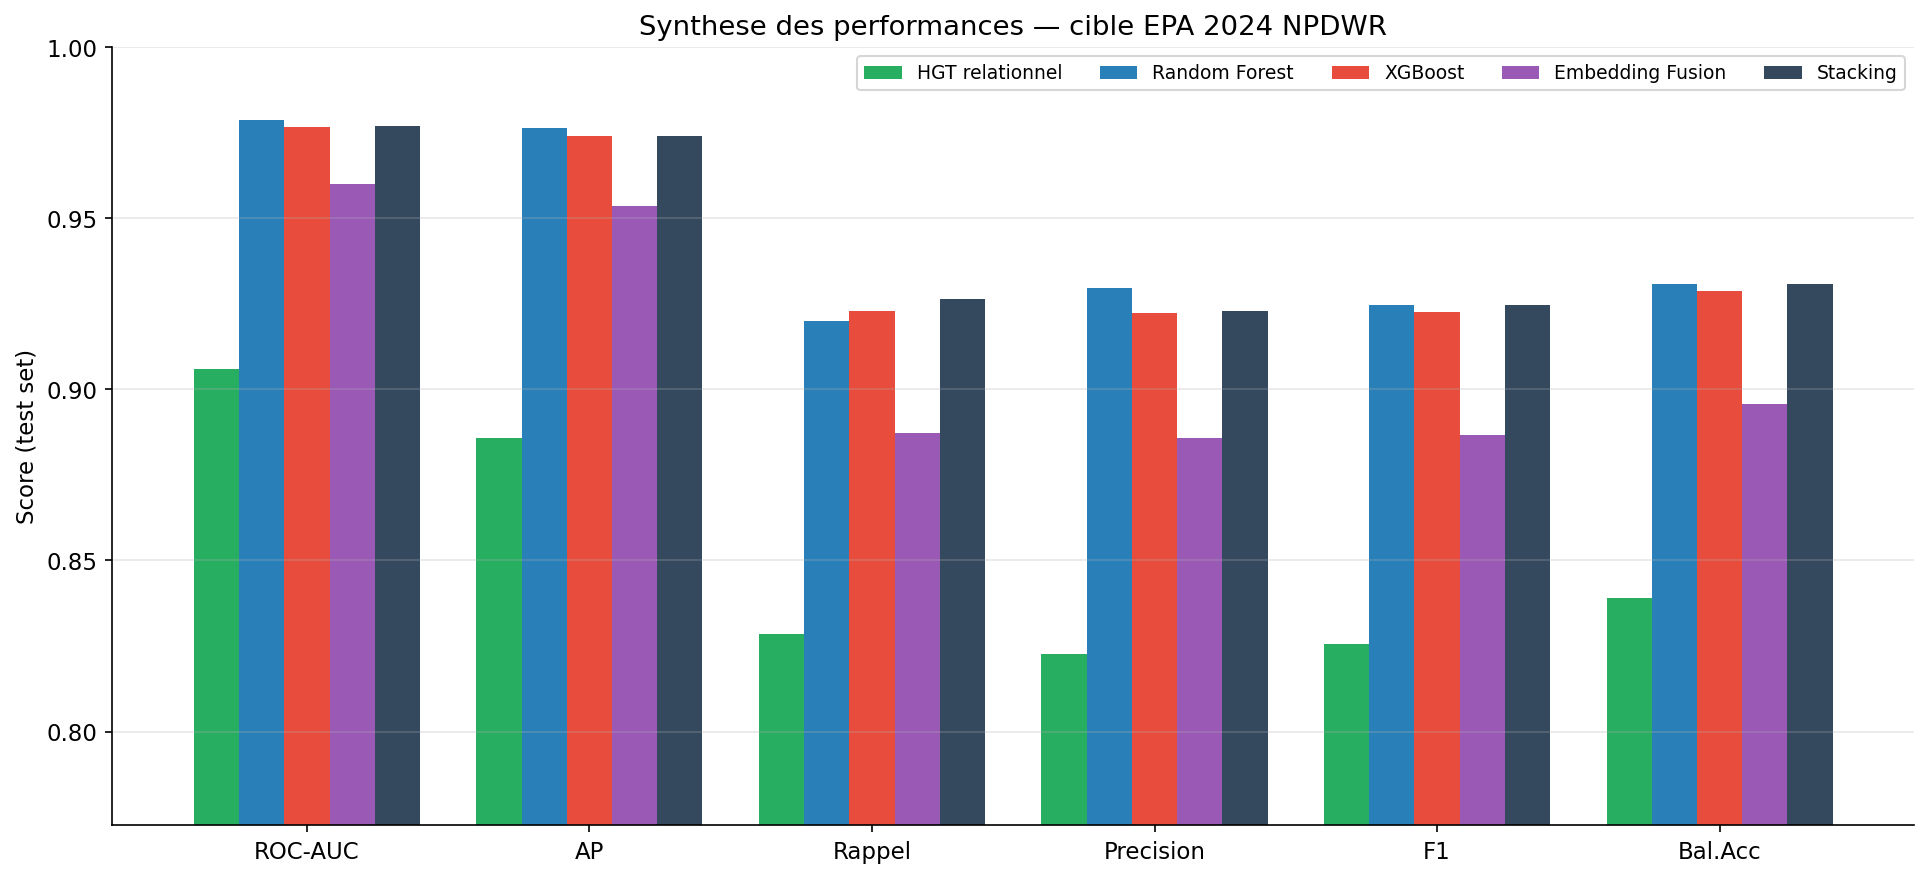
\includegraphics[width=0.95\linewidth]{Chap3/images/figures/fig27_dashboard.png}
    \caption{Tableau de bord comparatif des cinq mod\`eles (m\'etriques et matrices de confusion sur le jeu de test).}
    \label{fig:dashboard}
\end{figure}
On constate que les \'ecarts de F1 et d'exactitude \'equilibr\'ee confirment le classement~: l'architecture la plus \'elabor\'ee n'est pas la plus performante sur ce jeu.

Au-del\`a des m\'etriques de discrimination, un outil destin\'e \`a prioriser des forages \`a contr\^oler doit produire des probabilit\'es fiables~: si le mod\`ele annonce un risque de 70~\%, ce risque doit se r\'ealiser pour environ 70~\% des puits concern\'es. La figure~\ref{fig:calibration} confronte les probabilit\'es pr\'edites \`a la fr\'equence observ\'ee pour les cinq mod\`eles.

\begin{figure}[H]
    \centering
    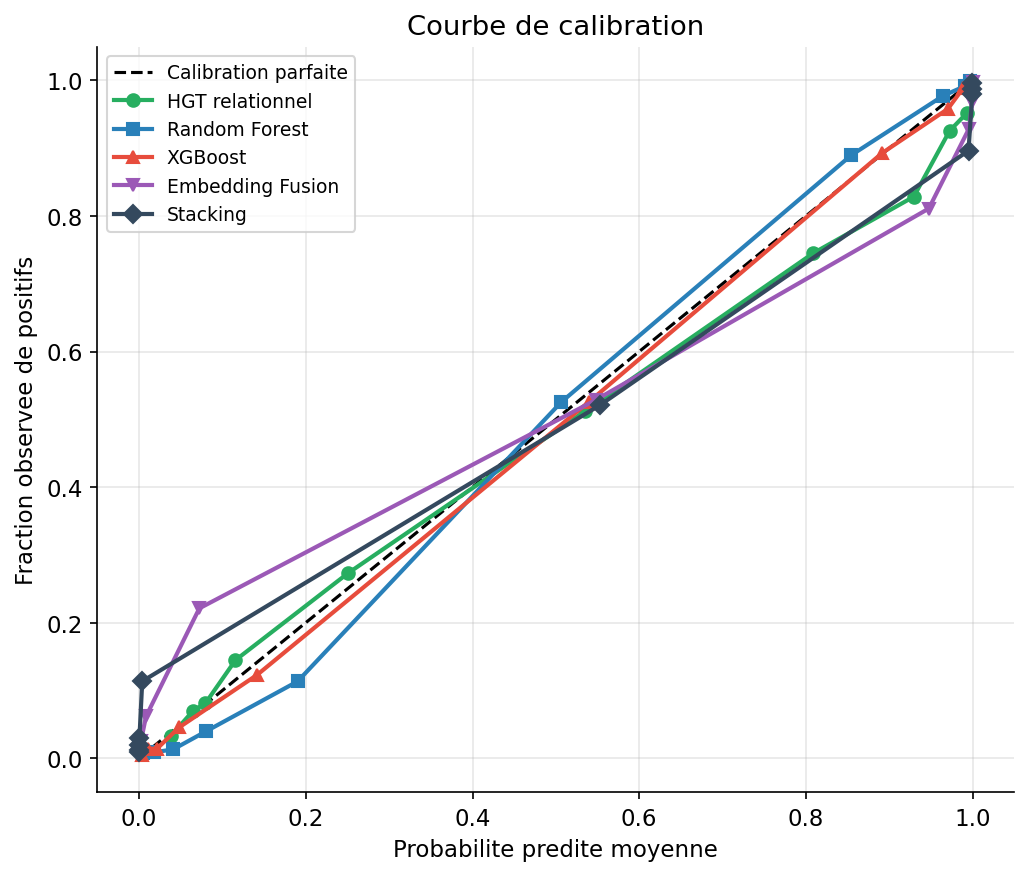
\includegraphics[width=0.82\linewidth]{Chap3/images/figures/fig25_calibration_all.png}
    \caption{Calibration des probabilit\'es de d\'epassement~: fr\'equence observ\'ee en fonction de la probabilit\'e pr\'edite pour les cinq mod\`eles (la diagonale repr\'esente une calibration parfaite).}
    \label{fig:calibration}
\end{figure}

On observe que la for\^et al\'eatoire et XGBoost, les plus performants en discrimination, pr\'esentent une calibration proche de la diagonale sur la majorit\'e de l'intervalle~; leurs probabilit\'es peuvent donc \^etre utilis\'ees directement pour classer des puits par ordre de risque d\'ecroissant. Le HGT et les mod\`eles hybrides s'en \'ecartent davantage, en particulier aux extr\'emit\'es, ce qui invite \`a les utiliser en classement relatif plut\^ot qu'en estimation absolue du risque. Pour un gestionnaire de surveillance, ce r\'esultat oriente le choix du mod\`ele~: la for\^et al\'eatoire offre le meilleur compromis entre discrimination et fiabilit\'e des probabilit\'es.

\mySubSection{Interpr\'etabilit\'e globale~: importance et concordance}{}
\label{sec:contrib-interp-globale}

L'analyse des importances de variables, men\'ee par valeurs de Shapley (section~\ref{sec:shapley-shap}), identifie les facteurs qui p\`esent le plus dans les pr\'edictions et mesure l'accord entre mod\`eles. Les variables les plus influentes sont la cat\'egorie du forage, la profondeur de la nappe, la densit\'e de sites de contamination dans le voisinage et la direction d'\'ecoulement. Ce sont des grandeurs de contexte hydrog\'eologique et de proximit\'e aux sources, et non des coordonn\'ees, ce qui est coh\'erent avec le retrait de la localisation. La figure~\ref{fig:importance} compare les importances par mod\`ele et la figure~\ref{fig:concordance} la concordance des rangs.

\begin{figure}[H]
    \centering
    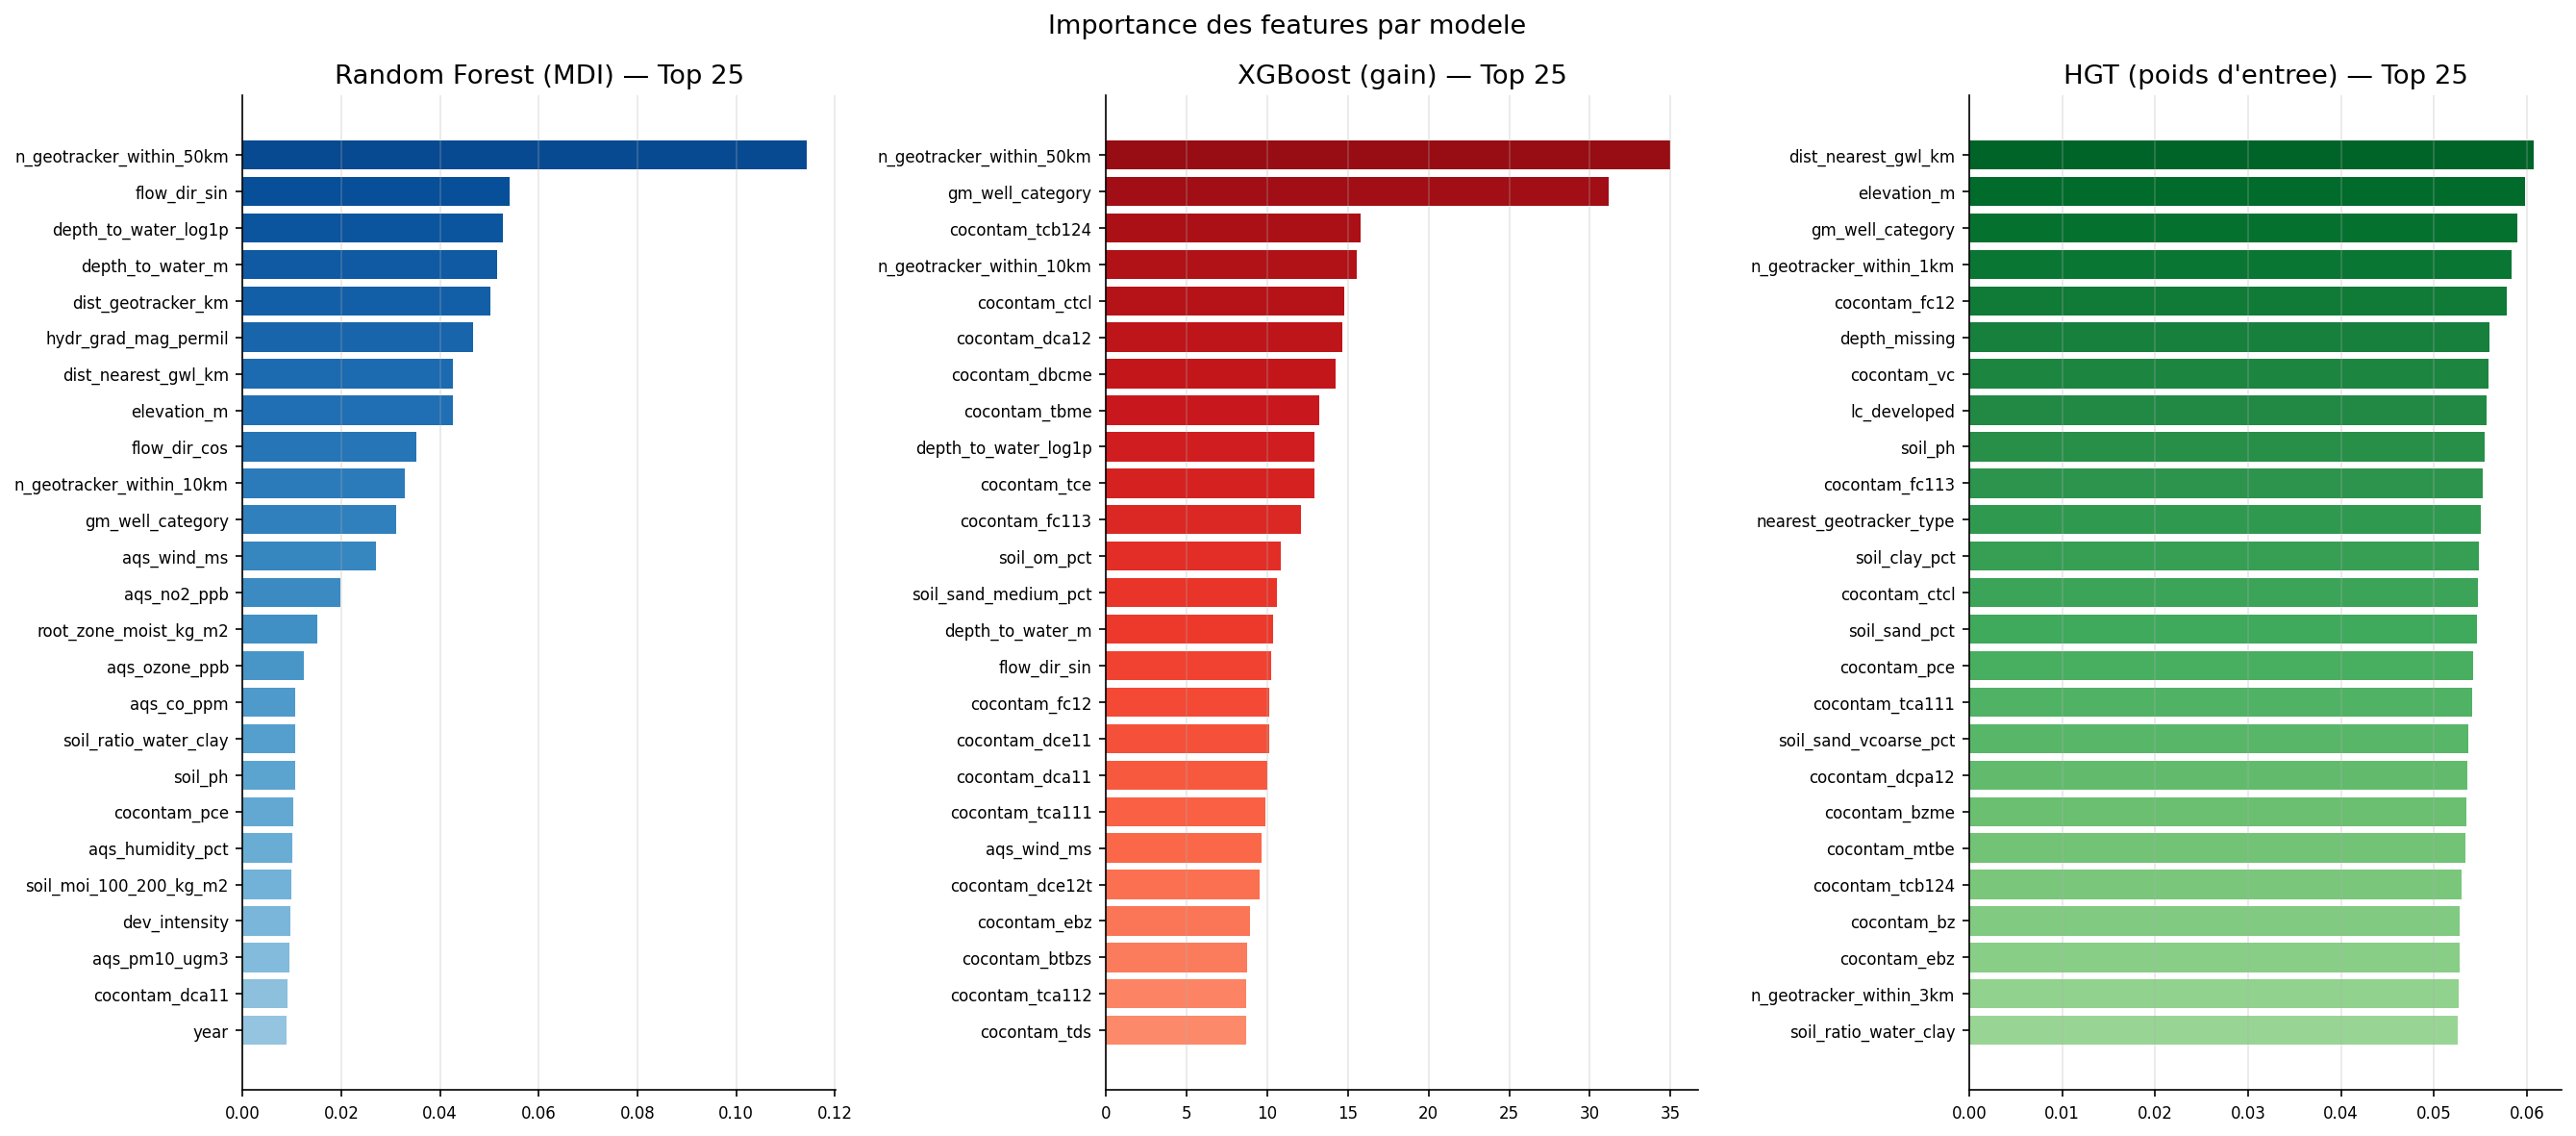
\includegraphics[width=0.95\linewidth]{Chap3/images/figures/fig40_importance_par_modele.png}
    \caption{Importance des variables par mod\`ele (Top 25, valeurs de Shapley).}
    \label{fig:importance}
\end{figure}

\begin{figure}[H]
    \centering
    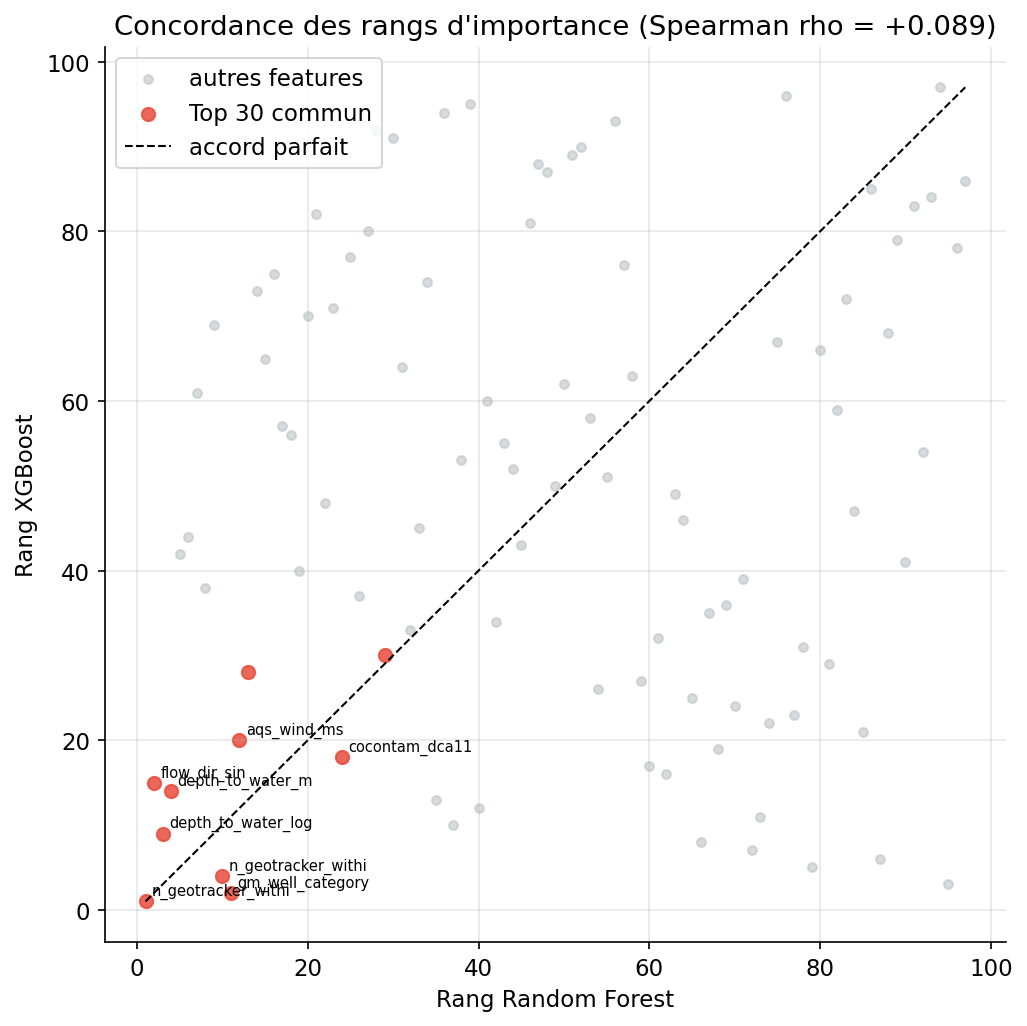
\includegraphics[width=0.75\linewidth]{Chap3/images/figures/fig41_concordance_rangs.png}
    \caption{Concordance des rangs d'importance entre mod\`eles.}
    \label{fig:concordance}
\end{figure}
On observe que les variables les plus influentes pour les mod\`eles tabulaires sont \texttt{n\_geotracker\_within\_50km} (rang~1 pour RF et XGBoost), la cat\'egorie du forage (\texttt{gm\_well\_category}, rang~2 pour XGBoost, rang~3 pour le HGT) et la profondeur de la nappe (\texttt{depth\_to\_water\_m}, rang~4 pour RF)~: pour un d\'ecideur, ces trois variables de proximit\'e et de contexte hydrog\'eologique constituent les facteurs diagnostiques prioritaires.

La concordance inter-mod\`eles, mesur\'ee par le coefficient de Spearman sur les rangs d'importance (Top~30), r\'ev\`ele un r\'esultat contre-intuitif. RF et XGBoost, pourtant presque aussi performants (AUC 0,979 vs 0,977), s'accordent tr\`es peu~: $\rho = 0{,}09$, avec seulement 10 variables communes. Deux mod\`eles presque \'equiperformants s'appuient donc sur des hi\'erarchies de variables sensiblement diff\'erentes. La paire XGBoost/HGT pr\'esente paradoxalement la concordance la plus \'elev\'ee ($\rho = 0{,}39$, avec 12 variables communes), alors que leurs performances respectives sont les plus \'eloign\'ees du banc. La concordance RF/HGT est la plus faible ($\rho = 0{,}05$, avec 7 variables communes). Ces chiffres indiquent que les trois mod\`eles lisent le probl\`eme par des canaux structurellement diff\'erents~; que cette diversit\'e ne se traduise pas en gain de stacking est un constat important, sugg\'erant que les canaux sont redondants plut\^ot que compl\'ementaires.

\mySubSection{Interpr\'etabilit\'e locale}{}
\label{sec:contrib-interp-locale}

Au-del\`a des tendances globales, chaque mod\`ele est expliqu\'e au niveau d'une pr\'ediction individuelle, sur un forage positif et un forage n\'egatif, par d\'ecomposition de la d\'ecision en contributions de variables (section~\ref{sec:shap-global-local}). Ces explications locales montrent quelles caract\'eristiques d'un forage ont pouss\'e la d\'ecision vers le d\'epassement ou vers la conformit\'e, ce qui rend une pr\'ediction d\'efendable aupr\`es d'un d\'ecideur, sans pour autant valoir preuve de causalit\'e. Nous illustrons ici l'interpr\'etabilit\'e locale sur la for\^et al\'eatoire, meilleur mod\`ele du banc.

La figure~\ref{fig:shap-local-rf-pos} d\'ecompose la d\'ecision pour un forage class\'e \`a risque~: chaque barre repr\'esente la contribution d'une variable (valeur de Shapley) \`a l'\'ecart entre la probabilit\'e pr\'edite et la probabilit\'e de r\'ef\'erence.

\begin{figure}[H]
    \centering
    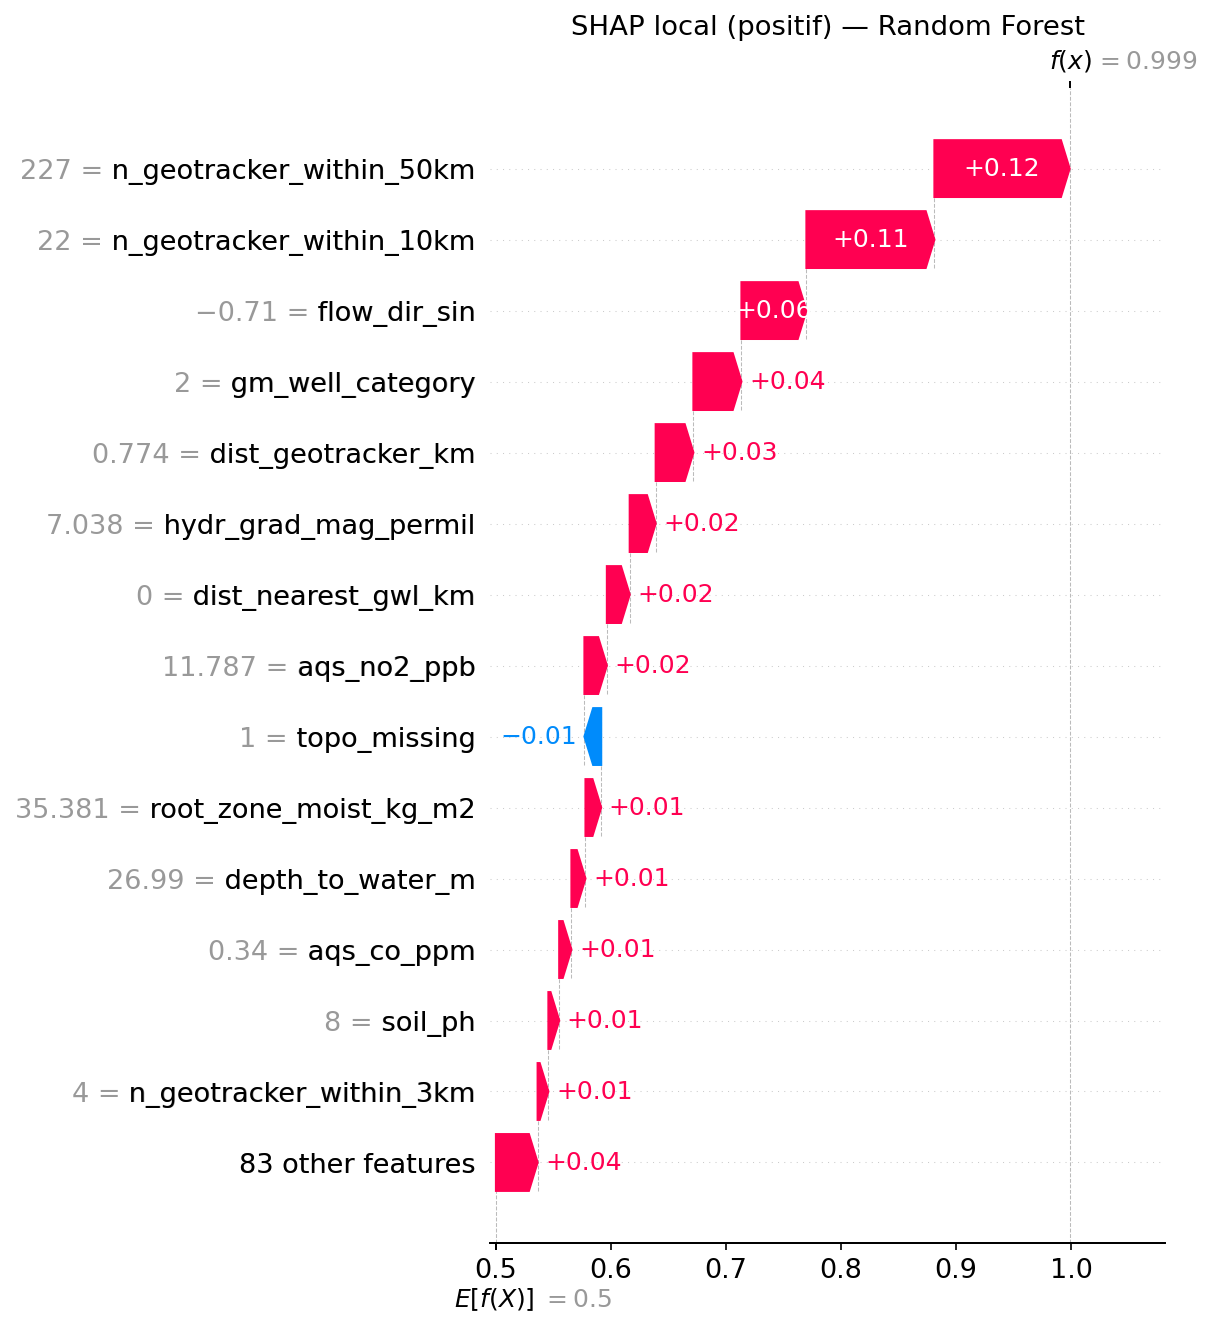
\includegraphics[width=0.85\linewidth]{Chap3/images/figures/fig06b_shap_local_rf_positif.png}
    \caption{Explication locale SHAP (diagramme \emph{waterfall}) de la for\^et al\'eatoire pour un forage class\'e \`a risque.}
    \label{fig:shap-local-rf-pos}
\end{figure}

On observe que la pr\'ediction est port\'ee par la densit\'e \'elev\'ee de sites de contamination \`a proximit\'e (\texttt{n\_geotracker\_within\_50km}), combin\'ee \`a la profondeur de la nappe et \`a la direction d'\'ecoulement~; ces variables accumulent la quasi-totalit\'e de la contribution positive et sont coh\'erentes avec les m\'ecanismes hydrog\'eologiques de migration des PFAS.

La figure~\ref{fig:shap-local-rf-neg} pr\'esente le cas sym\'etrique, un forage pr\'edit conforme.

\begin{figure}[H]
    \centering
    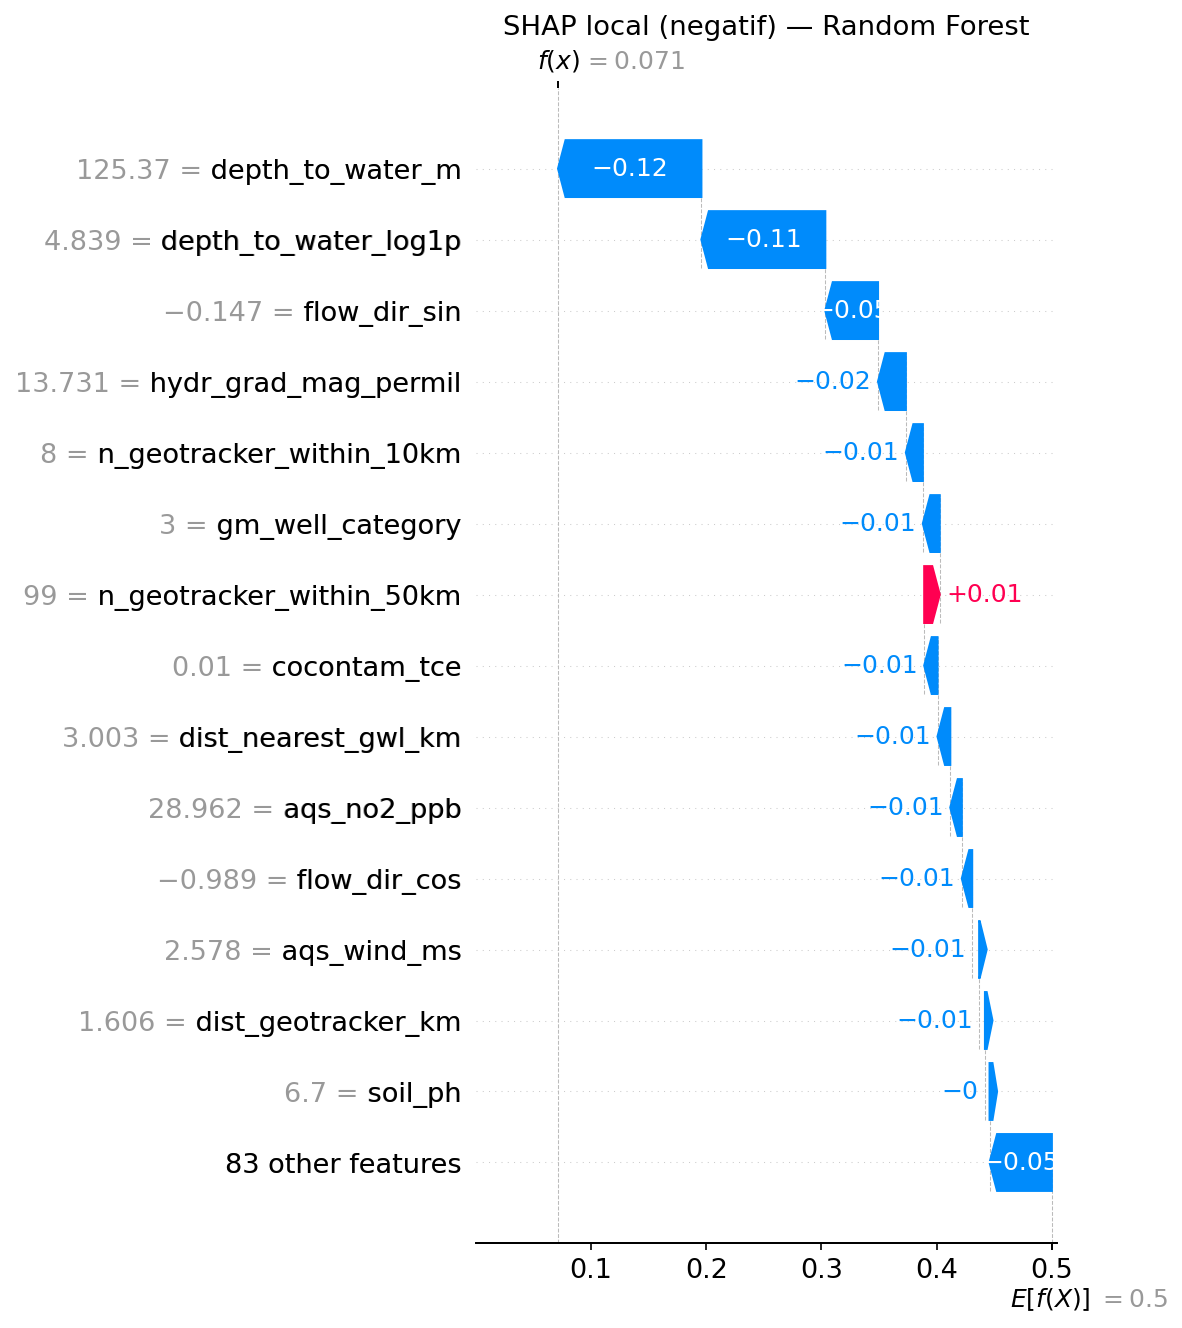
\includegraphics[width=0.85\linewidth]{Chap3/images/figures/fig06b_shap_local_rf_negatif.png}
    \caption{Explication locale SHAP (diagramme \emph{waterfall}) de la for\^et al\'eatoire pour un forage class\'e conforme.}
    \label{fig:shap-local-rf-neg}
\end{figure}

On constate que les m\^emes variables jouent dans le sens inverse~: la faible densit\'e de sites \`a proximit\'e et une profondeur de nappe \'elev\'ee sont les arguments principaux en faveur de la conformit\'e. La coh\'erence des facteurs d\'eterminants entre les deux cas renforce la cr\'edibilit\'e du mod\`ele~: ses d\'ecisions s'appuient sur des grandeurs physiquement interpr\'etables, ce qui est une condition n\'ecessaire pour en faire un outil d'aide \`a la priorisation de la surveillance.

\mySubSection{Sous le capot du HGT}{}
\label{sec:contrib-hgt-capot}

\`A des fins p\'edagogiques, le fonctionnement du graphe relationnel est expos\'e pas \`a pas. Les figures~\ref{fig:site-neighborhood} et~\ref{fig:well-neighborhood} donnent \`a voir la structure h\'et\'erog\`ene effectivement construite autour d'un site de contamination puis d'un forage, et la figure~\ref{fig:embeddings-2d} projette en deux dimensions les embeddings appris.

\begin{figure}[H]
    \centering
    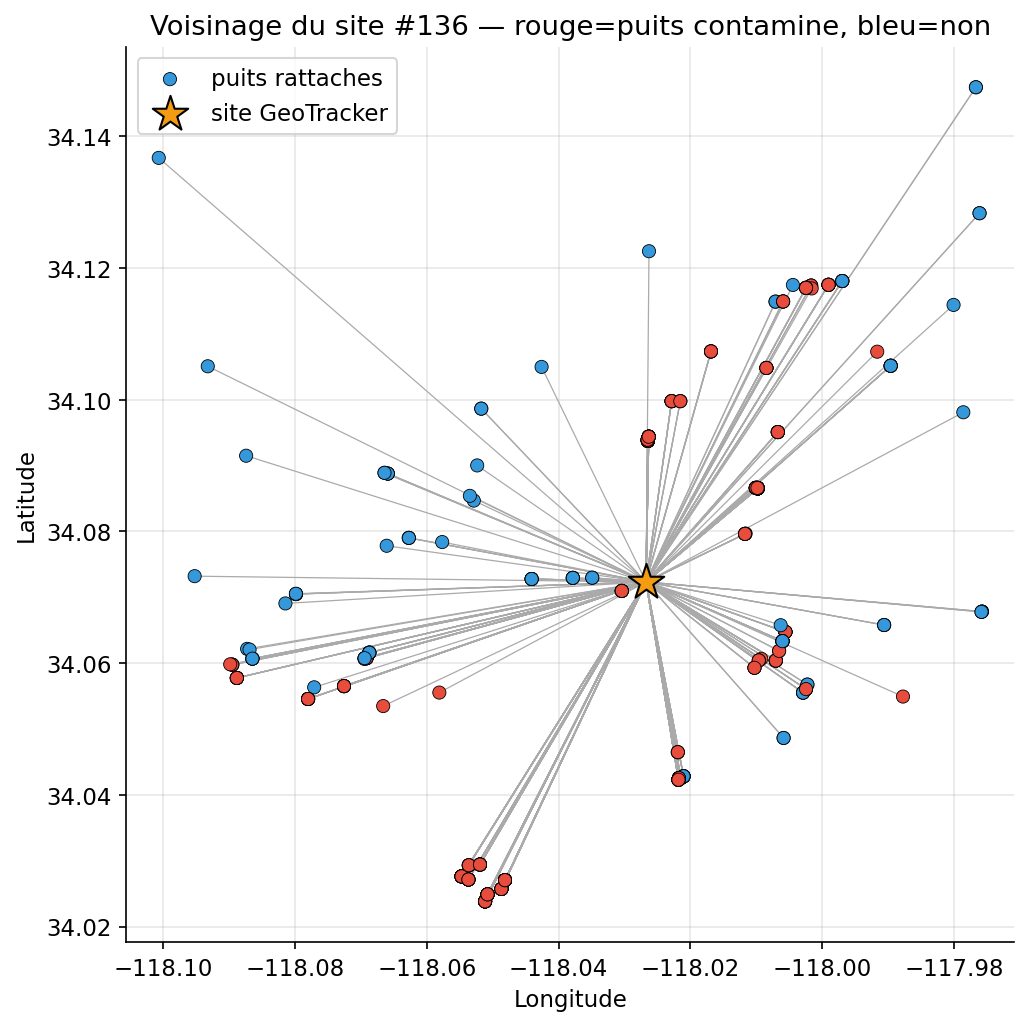
\includegraphics[width=0.8\linewidth]{Chap3/images/figures/fig30_site_neighborhood.png}
    \caption{Voisinage d'un site de contamination dans le graphe h\'et\'erog\`ene.}
    \label{fig:site-neighborhood}
\end{figure}

\begin{figure}[H]
    \centering
    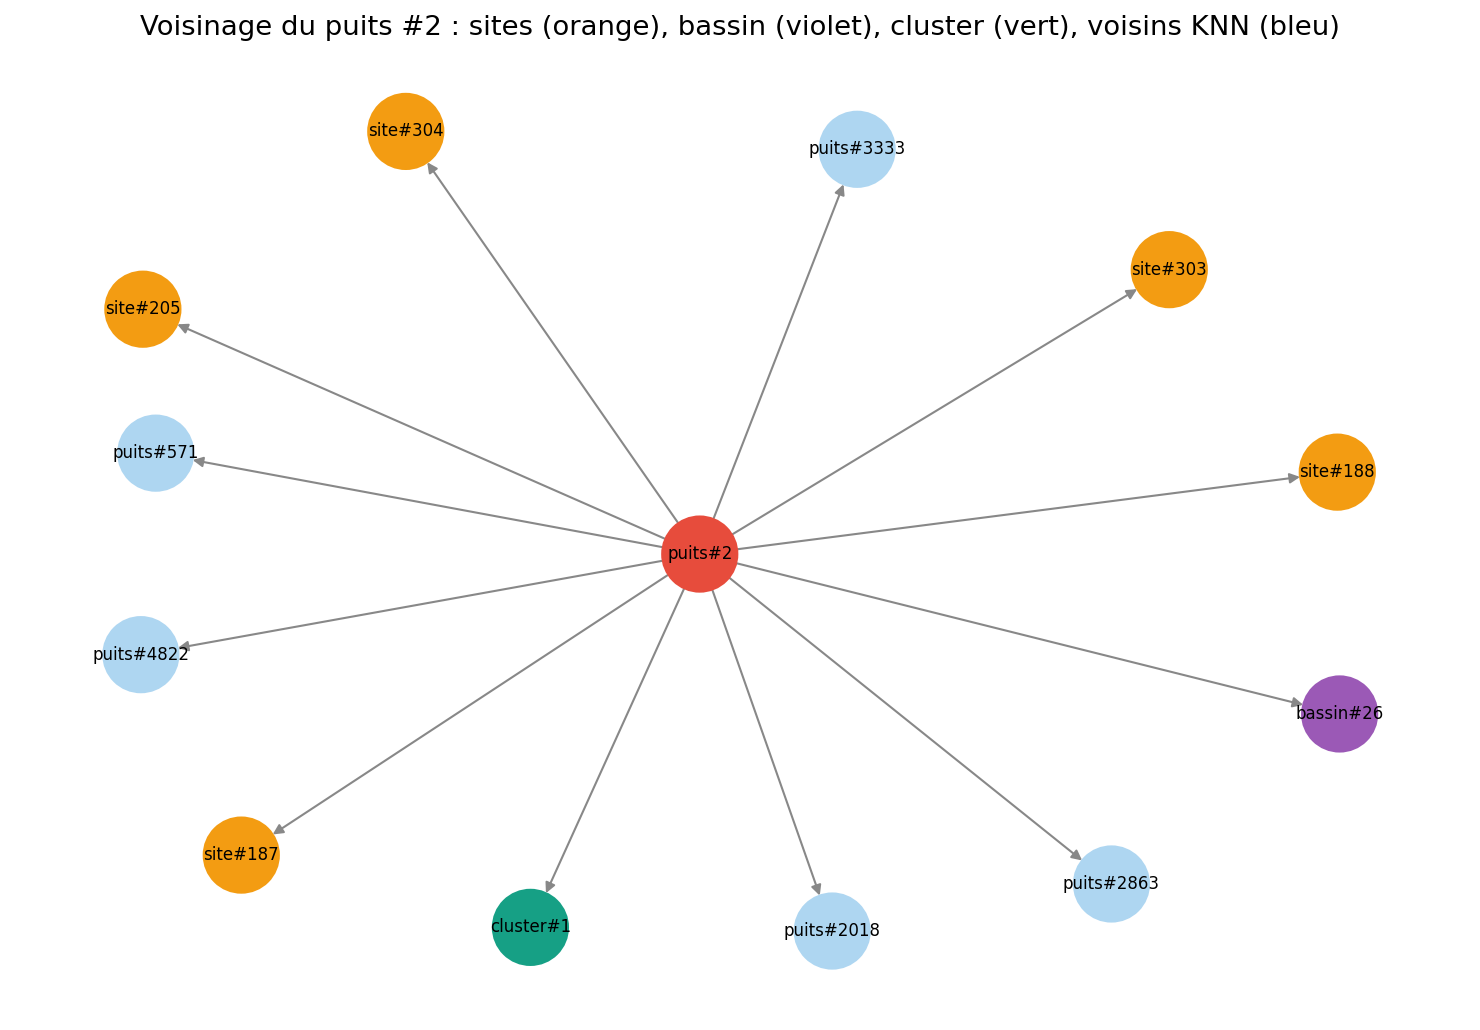
\includegraphics[width=0.8\linewidth]{Chap3/images/figures/fig31_well_neighborhood.png}
    \caption{Voisinage d'un forage~: ar\^etes vers les entit\'es partag\'ees et les voisins spatiaux.}
    \label{fig:well-neighborhood}
\end{figure}

\begin{figure}[H]
    \centering
    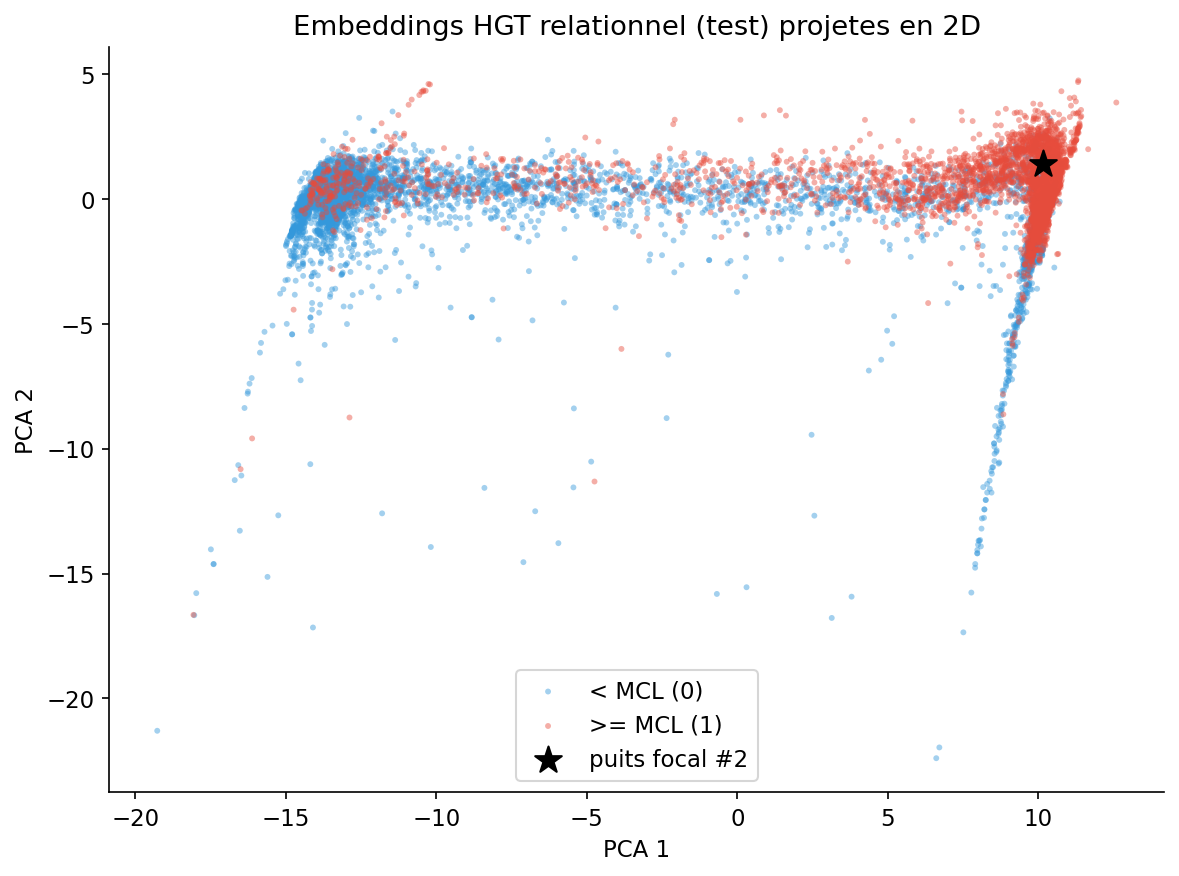
\includegraphics[width=0.8\linewidth]{Chap3/images/figures/fig33_hgt_embeddings_2d.png}
    \caption{Projection en deux dimensions des embeddings appris par le HGT, color\'ee par classe.}
    \label{fig:embeddings-2d}
\end{figure}
On observe que la projection s\'epare partiellement les forages \`a risque des autres~: la s\'eparation apprise est r\'eelle mais moins nette que celle que procurent les variables de contexte, ce qui explique le retrait du HGT en performance.

\mySubSection{Cartographie des pr\'edictions}{}
\label{sec:contrib-carte}

Les pr\'edictions du meilleur mod\`ele sont restitu\'ees spatialement (figure~\ref{fig:map-predictions}), ce qui permet de confronter les zones jug\'ees \`a risque \`a la g\'eographie connue de la contamination.

\begin{figure}[H]
    \centering
    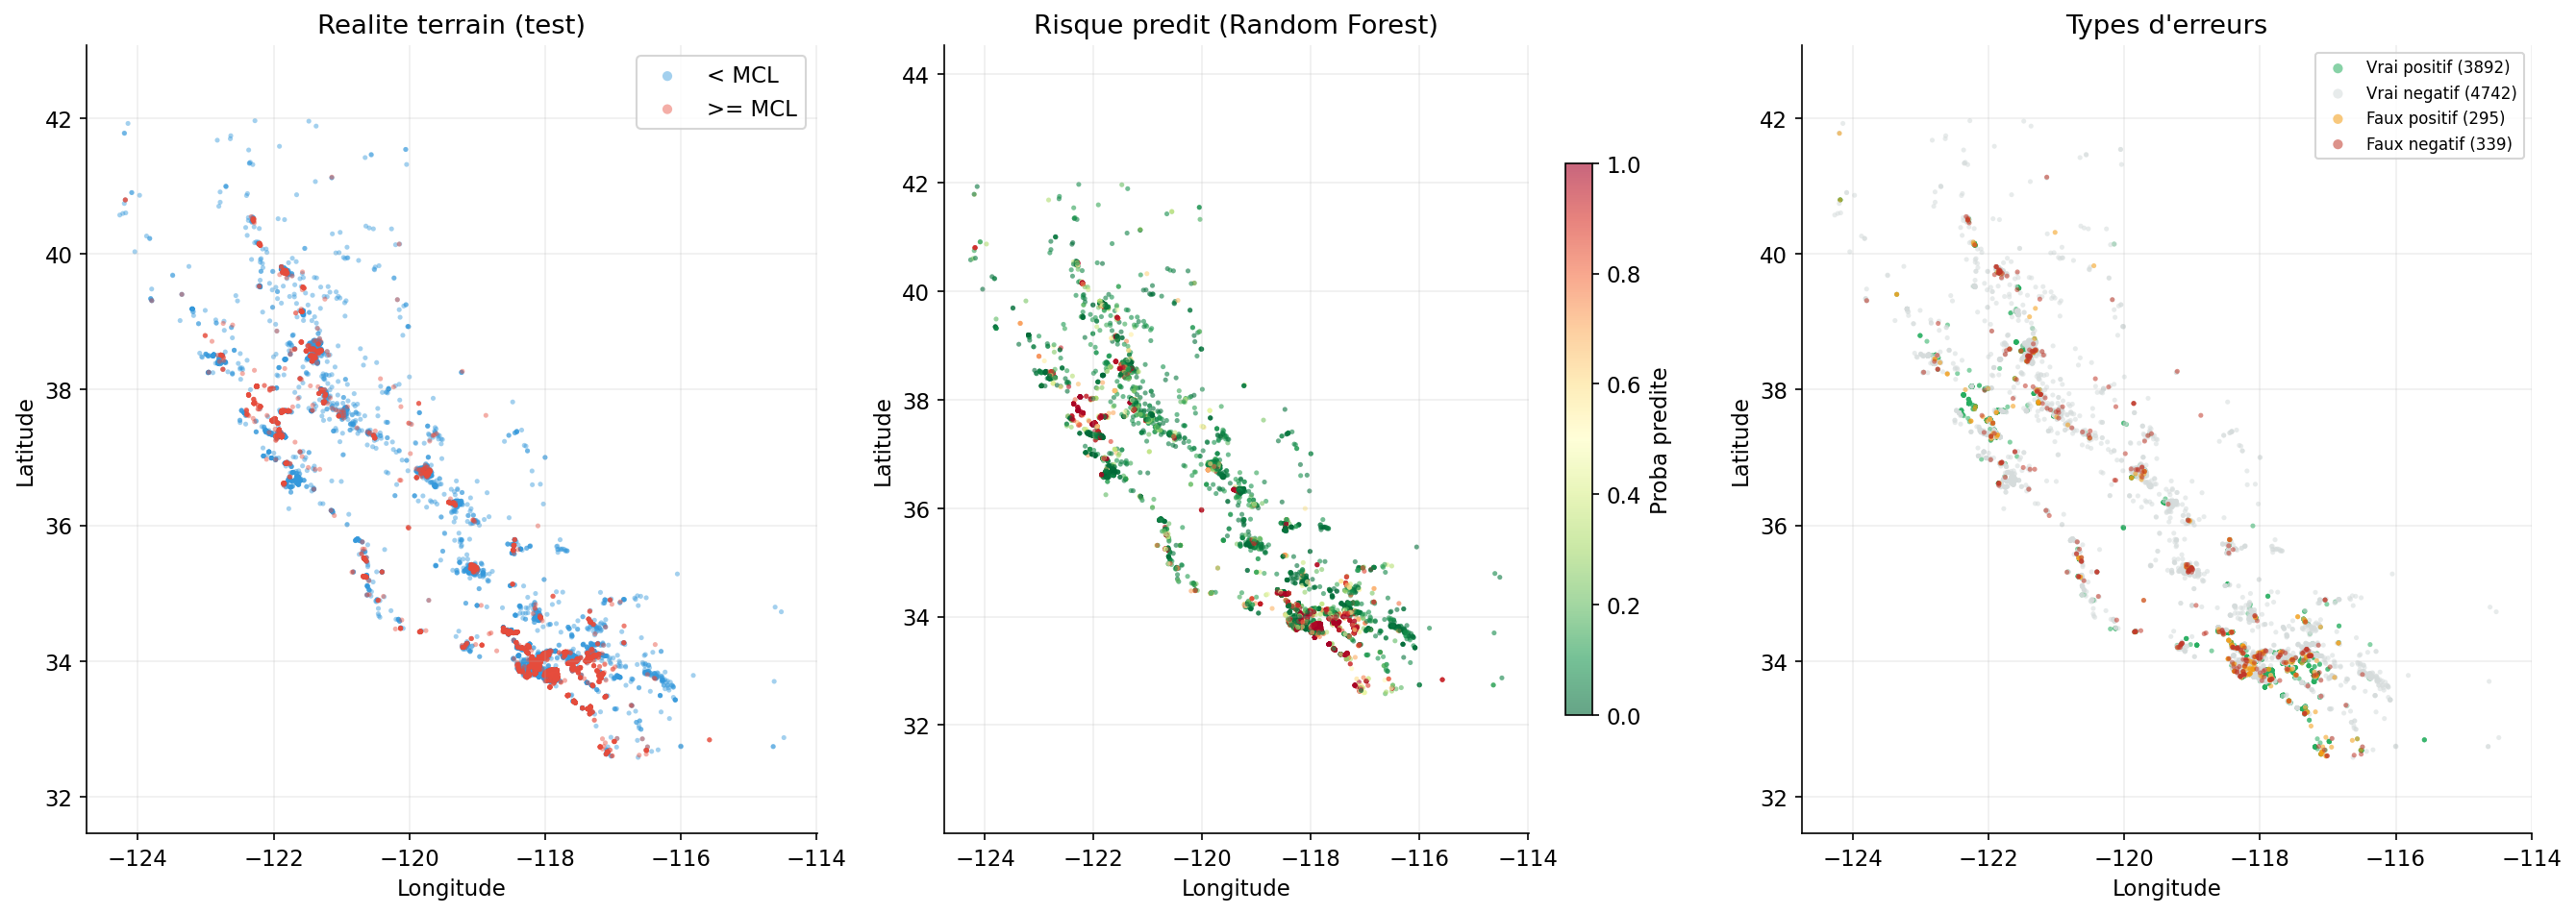
\includegraphics[width=0.8\linewidth]{Chap3/images/figures/fig28_map_predictions.png}
    \caption{Carte des pr\'edictions du meilleur mod\`ele sur la Californie.}
    \label{fig:map-predictions}
\end{figure}
On constate que les zones \`a risque pr\'edites co\"incident avec les secteurs historiquement contamin\'es, sans concentration manifeste de faux positifs, ce qui appuie l'usage du mod\`ele comme outil de priorisation de la surveillance.

\mySubSection{Discussion}{}
\label{sec:contrib-discussion}

Le principal enseignement est que, sur ce jeu de donn\'ees, les variables de contexte produites par \texttt{geoenrich} portent l'essentiel du signal pr\'edictif~: des mod\`eles tabulaires classiques, priv\'es de toute coordonn\'ee, atteignent une discrimination \'elev\'ee. Le pari de porter la g\'eographie par la structure d'un graphe plut\^ot que par des variables n'am\'eliore pas la pr\'ediction, et les hybrides ne d\'egagent pas de compl\'ementarit\'e exploitable. L'analyse des importances du m\'eta-classifieur du stacking le quantifie directement~: la probabilit\'e pr\'edite par le HGT (\texttt{hgt\_p1}) ne repr\'esente que 0,5~\% du poids d\'ecisionnel, contre 41~\% pour la probabilit\'e XGBoost et 7~\% pour celle de RF~; le produit crois\'e RF$\times$XGBoost (\texttt{prod\_xr}) concentre \`a lui seul 45~\% de l'importance. Le m\'eta-classifieur apprend donc \`a ignorer le HGT et \`a arbitrer presque exclusivement entre les deux mod\`eles tabulaires, ce qui explique que le stacking ne d\'epasse pas la for\^et al\'eatoire. Ce r\'esultat, n\'egatif au sens o\`u l'architecture la plus \'elabor\'ee n'est pas la plus performante, a sa valeur~: il montre qu'un enrichissement de contexte soign\'e peut rendre superflue une mod\'elisation relationnelle plus lourde.

Une limite m\'ethodologique m\'erite d'\^etre signal\'ee concernant les co-contaminants (\texttt{cocontam\_*}, 44 colonnes). Ces variables encodent la pr\'esence d'autres polluants mesur\'es dans les m\^emes programmes de surveillance que les PFAS~; or, les programmes de surveillance sont souvent d\'eclench\'es dans des zones d\'ej\`a suspect\'ees de contamination. Contrairement aux concentrations PFAS elles-m\^emes, les co-contaminants ne d\'efinissent pas la cible de fa\c{c}on d\'eterministe, mais ils peuvent en constituer un proxy indirect par biais de s\'election. Leur impact devra \^etre \'evalu\'e par une analyse de sensibilit\'e dans les travaux futurs.

Ces conclusions doivent \^etre temp\'er\'ees par une limite d'\'evaluation. Les performances rapport\'ees reposent sur un d\'ecoupage stratifi\'e al\'eatoire, qui ne teste pas la g\'en\'eralisation \`a des r\'egions enti\`erement non vues. Or la contamination PFAS est fortement auto-corr\'el\'ee dans l'espace, et m\^eme des variables de contexte (densit\'e de sites, proximit\'e) encodent indirectement la position~: une partie de la performance pourrait donc tenir \`a une auto-corr\'elation spatiale r\'esiduelle plut\^ot qu'\`a des m\'ecanismes transf\'erables. La validation crois\'ee spatiale par blocs est l'outil qui permettrait de mesurer ce risque, et son ex\'ecution constitue une priorit\'e pour consolider les conclusions. En l'absence de ce test, les comparaisons entre mod\`eles restent valides, puisqu'elles s'effectuent \`a protocole identique, mais le niveau absolu de performance doit \^etre interpr\'et\'e comme une borne sup\'erieure optimiste.

Par rapport \`a l'\'etat de l'art californien, Dong et al.~\cite{dong2024pfas} constituent la r\'ef\'erence la plus proche~: m\^eme corpus GAMA, m\^eme mode pr\'edictif strict (variables contextuelles exclusivement, sans concentration PFAS en entr\'ee). Deux diff\'erences structurelles emp\^echent toute comparaison chiffre \`a chiffre. D'une part, la cible change de cadre r\'eglementaire~: Dong et al. visent le seuil conjoint de 70~ng/L des recommandations EPA 2016, ce travail applique le NPDWR 2024 qui abaisse les seuils \`a 4~ng/L pour le PFOA et le PFOS et introduit le crit\`ere de m\'elange (HI)~; ce changement modifie la pr\'evalence des positifs et rend les m\'etriques non directement comparables. D'autre part, les paradigmes d'apprentissage diff\`erent~: Dong et al. mobilisent un pseudo-\'etiquetage semi-supervis\'e pour exploiter les 90~\% de puits sans analyse compl\`ete, et organisent la pr\'ediction en cha\^ine de classifieurs sur 35 analytes distincts~; ce travail est purement supervis\'e et formule la t\^ache comme un probl\`eme binaire unique sur la non-conformit\'e r\'eglementaire. L'apport architectural sp\'ecifique est l'introduction du HGT pour mod\'eliser la structure relationnelle spatiale entre forages, une direction absente de la litt\'erature PFAS publi\'ee (lacune~L1, section~\ref{sec:chap2-lacunes})~; les r\'esultats montrent que ce b\'en\'efice attendu ne s'est pas mat\'erialis\'e sur ce corpus, ce qui est en soi une information utile pour orienter de futurs travaux sur la structure relationnelle des r\'eseaux de surveillance.

% =========================================================
\mySection{Synth\`ese}{}
\label{sec:synthese-chap3}
% =========================================================

Ce chapitre a pr\'esent\'e une double contribution \`a la pr\'ediction du risque PFAS dans les eaux souterraines californiennes. La premi\`ere est un outil, \texttt{geoenrich}, moteur d'enrichissement g\'eospatial organis\'e en trois couches et fond\'e sur un contrat d'entr\'ee minimal qui s\'epare le \emph{o\`u/quand} universel de la charge utile \'etudi\'ee. Appliqu\'e \`a la base \texttt{wells\_pfas\_cleaned} reconstruite \`a partir des donn\'ees ouvertes californiennes (46\,338 pr\'el\`evements sur environ 11\,300 puits, d'avril 2016 \`a janvier 2026), il porte le jeu \`a 217 colonnes, dont les variables de contexte ajout\'ees par l'enrichissement spatial sont presque toutes compl\`etes (88 colonnes renseign\'ees \`a 100~\%). La seconde contribution est un banc de cinq mod\`eles, deux mod\`eles tabulaires de r\'ef\'erence, un transformeur de graphe h\'et\'erog\`ene et deux mod\`eles hybrides, \'evalu\'es \`a protocole identique et en mode pr\'edictif sur ce jeu enrichi.

L'enseignement principal est que les variables de contexte produites par \texttt{geoenrich} portent l'essentiel du signal pr\'edictif~: des mod\`eles tabulaires priv\'es de toute coordonn\'ee atteignent une discrimination \'elev\'ee (ROC-AUC proche de 0,98), tandis que structurer la g\'eographie dans un graphe relationnel n'am\'eliore pas la pr\'ediction et que les hybrides ne d\'egagent pas de compl\'ementarit\'e. Deux limites tracent les perspectives. D'une part, la r\'eutilisabilit\'e de \texttt{geoenrich} sur un autre polluant ou une autre r\'egion reste \`a confirmer par une application empirique \`a un nouveau jeu d'observations. D'autre part, l'\'evaluation repose sur un d\'ecoupage qui ne teste pas la g\'en\'eralisation \`a des zones non vues~; l'ex\'ecution de la validation crois\'ee spatiale par blocs est la priorit\'e imm\'ediate pour distinguer la part de signal transf\'erable de l'auto-corr\'elation spatiale r\'esiduelle. Ces deux chantiers prolongent le travail sans en remettre en cause les acquis~: un outil d'enrichissement r\'eutilisable et une comparaison rigoureuse et interpr\'etable de mod\`eles de pr\'ediction de la contamination.
